\documentclass[xcolor={x11names,svgnames}]{beamer}
\setbeamerfont{note page}{size=\tiny} % default = small 

\newcommand{\heading}{\frametitle}

\usecolortheme{rose}
\setbeamertemplate{footline}{}
\setbeamertemplate{navigation symbols}{}

\usepackage{amsmath, amssymb, amsthm}
\usepackage{epsfig}
\usepackage[utf8]{inputenc}
\usepackage[french]{babel}
\usepackage[T1]{fontenc}
\usepackage[normalem]{ulem}   
\usepackage{framed}   
\usepackage{tabularx}
\usepackage{url}
\usepackage{psfrag}
\usepackage{alltt}
\usepackage{minted}
\usepackage{tikz}
\usetikzlibrary{positioning}
\usetikzlibrary{calc}
\usetikzlibrary{decorations}
\usetikzlibrary{decorations.pathmorphing}
\usetikzlibrary{decorations.pathreplacing}
\usetikzlibrary{shapes.multipart}


\definecolor{red}{rgb}{1, 0, 0}
\definecolor{Green}{rgb}{0, 0.6, 0}
\definecolor{Purple}{rgb}{0.75, 0, 0.25}

%\newcommand{\red}{\color{red}}
\newcommand{\po}{\xrightarrow{po}}
\newcommand{\net}{\xrightarrow{net}}
\newcommand{\hb}{{\color{blue}\xrightarrow{\texttt{hb}}}}
\newcommand{\rf}{{\color{Green}\xrightarrow{\texttt{rf}}}}
\newcommand{\mo}{{\color{orange}\xrightarrow{\texttt{mo}}}}
\newcommand{\rb}{{\color{Purple}\xrightarrow{\texttt{rb}}}}
\newcommand{\rmw}{{\color{gray}\xrightarrow{\texttt{rmw}}}}
\newcommand{\eco}{{\color{red}\xrightarrow{\texttt{eco}}}}


\newcommand{\blue}[1]{{\color{Blue}#1}}
\newcommand{\green}[1]{{\color{LimeGreen}#1}}
\newcommand{\red}[1]{{\color{red}#1}}
\newcommand{\tikzmat}[2] {
\draw[thick] let \p1 = (#1 |- #2),
                 \p2 = (#2 |- #1) in
   ($ (#1) + (0.05,-0.1) $) -- ++(-0.15, 0)  -- ($ (\p1) + (-0.1,0.1) $) -- ++(0.15,0)
   ($ (\p2) + (-0.05,-0.1) $) -- ++(0.15, 0) -- ($ (#2) + (0.1,0.1) $) -- ++(-0.15,0);
}


\setminted{fontsize=\scriptsize}

\newtheorem{defi}{Définition}
\newtheorem{lemm}{Lemme}
\newtheorem{exem}{Exemple}
\newtheorem{theor}{Théorème}
\newtheorem{algo}{Algorithme}

\newcommand{\fixme}[1]{{\bf #1}}
\newcommand{\textstruct}[1]{{\color{beamerstructure} #1}}
\newcommand{\textstructbf}[1]{{\color{beamerstructure} \textbf{#1}}}

\newcommand{\mynote}[1]{\note<1>[item]{#1}}

\usepackage{fontspec}

\setsansfont{PalatinoSansLTPro}[
   Path = /home/charles/charles_work/fonts/PalatinoSans/, 
   Extension      = .otf,
   UprightFont    = *-Regular,
   BoldFont= *-Bold ,
   ItalicFont = *-Italic,
   BoldItalicFont = *-BoldIta
]


\author[C.~Bouillaguet]{Charles Bouillaguet \newline
  {\small \texttt{charles.bouillaguet@lip6.fr}}}

\title{OpenMP suite}

\begin{document}


\begin{frame}
  \titlepage
\end{frame}


%%%%%%%%%%%%%%%%%%%%%%%%%%%%%%%%%%%%%%%%%%%%%%%%%%%%%%%%%%%%%%%%%%%%%%%
\begin{frame}[fragile]
  \frametitle{Retour sur un exemple}

%  \small
  \begin{columns}[t]
  \column{5.5cm}
\begin{block}{Programme}
\begin{minted}{C}
#include <stdio.h>
  
int main()
{
  int c = 0;
  #pragma omp parallel for
  for (int i = 0; i < 100000; i++) { 
       c++; 
  }
  printf("c=%d\n", c);
}
\end{minted}
\end{block}
    
    
    \column{4.5cm}
\begin{block}{Exécution}    
\footnotesize
\begin{verbatim}
$ ./a.out
c=15074
\end{verbatim}
\end{block}    
  \end{columns}
\end{frame}



%%%%%%%%%%%%%%%%%%%%%%%%%%%%%%%%%%%%%%%%%%%%%%%%%%%%%%%%%%%%%%%%%%%%%%%
\begin{frame}[fragile]
  \frametitle{Entrelacement des incrémentations}
  \framesubtitle{Architectures \emph{Load-Store}}

  \bigskip
  
  \begin{center}
    \begin{tikzpicture}
      \path[red,dotted,use as bounding box] (-2,-1.5) rectangle (8,3);

      % "RAM"
      \begin{scope}[yshift=1.75cm, every node/.style={anchor=base}]
        \path (1, 0.4) -- node[above=2mm] {RAM} (5, 0.4);
        \draw[thick] (1, -0.2) rectangle (5, 0.4);
        \node<1-10> at (3, 0) {$c = 42$};
        \node<11-12> at (3, 0) {$c = 43$};
        \node<13>[text=red] at (3, 0) {$c = 43$};
      \end{scope}

      \node (CPU1) at (0, 0) {
\includegraphics[width=2cm]{cpu_clipart.png}};
      \node<3-6>[draw,anchor=east,font=\scriptsize] at (-1.5, 0) {\texttt{\%rax = 42}};
      \node<7->[draw,anchor=east,font=\scriptsize] at (-1.5, 0) {\texttt{\%rax = 43}};
      
      \node (CPU2) at (6, 0) {
\includegraphics[width=2cm]{cpu_clipart.png}};
      \node<5-8>[draw,anchor=west,font=\scriptsize] at (7.5, 0) {\texttt{\%rax = 42}};
      \node<9->[draw,anchor=west,font=\scriptsize] at (7.5, 0) {\texttt{\%rax = 43}};


      % flèches RAM <--> CPU
      \draw<2>[thick,<-] (CPU1) |- (0.9, 1.85);
      \draw<10>[thick,->] (CPU1) |- (0.9, 1.85);

      \draw<4>[thick,<-] (CPU2) |- (5.1, 1.85);
      \draw<12>[thick,->] (CPU2) |- (5.1, 1.85);


      \node<6> at (0, -1.3) {\texttt{add \%rax, 1}};
      \node<8> at (6, -1.3) {\texttt{add \%rax, 1}};
\end{tikzpicture}
\end{center}
\end{frame}

%%%%%%%%%%%%%%%%%%%%%%%%

\begin{frame}[fragile]

  \begin{columns}[t]
  \column{5.5cm}
  \centering\includegraphics[width=1cm]{triste.png}

  \begin{block}{Mauvais}
\begin{minted}{C}
#include <stdio.h>
  
int main()
{
  int c = 0;
  #pragma omp parallel for
  for (int i = 0; i < 100000; i++) { 

    c++; 
  }
  printf("c=%d\n", c);
}
\end{minted}
\end{block}
    
    
    \column{5.5cm}
    \centering\includegraphics[width=1cm]{content.png}

  \begin{block}{Bon}
\begin{minted}{C}
#include <stdio.h>
  
int main()
{
  int c = 0;
  #pragma omp parallel for
  for (int i = 0; i < 100000; i++) { 
    #pragma omp atomic update
    c++; 
  }
  printf("c=%d\n", c);
}
\end{minted}
\end{block}
  \end{columns}

  \begin{alertblock}{Architectures \emph{load-store} :}
    \texttt{x++}, \texttt{x += 10}, etc. ne \textbf{sont pas atomiques}.
  \end{alertblock}

\end{frame}

%%%%%%%%%%%%%%%%%%%%%%%%%%%%%%%%%%%%%%%%%%%%%%%%%%%%%%%

\begin{frame}[label=golden_rule]
%  \frametitle{}

  \begin{center}
    \Huge \bf \alert{Règle d'or de la \\ programmation multithreads}
  \end{center}

  \bigskip
  
  {\Large \textbf{Tous} les accès potentiellement conflictuels${}^*$ aux variables partagées doivent être protégés (\texttt{atomic}, \texttt{critical}, ...).}

  \bigskip

  $*$ au moins l'un d'entre eux est une écriture.  
\end{frame}

%%%%%%%%%%%%%%%%%%%%%%%%%%%%%%%%%%%%%%%%%%%%%%%%%%%%%%

\section{Atomic vs Reduce}


\begin{frame}[fragile]
  \frametitle{\texttt{\#pragma omp atomic} n'est pas la panacée}
  \framesubtitle{Exemple : somme des éléments d'un tableau}

\begin{minted}{C}
int sum = 0;
for (int i = 0; i < n; i++)
    sum += A[i];
\end{minted}

      \bigskip
      
      \Large \alert{$T = 5.95$s} \qquad ($n = 10^{10}$)


      \vspace{1cm}
      
  \begin{columns}
    \begin{column}{0.4\textwidth}
\begin{minted}{C}
int sum = 0;
#pragma omp parallel for
for (int i = 0; i < n; i++)
    #pragma omp atomic
    sum += A[i];
\end{minted}

      \bigskip
      
      \uncover<2>{ \Large \alert{$T \geq 200$s !!!}}
      
    \end{column}
    \begin{column}{0.6\textwidth}
\begin{minted}{C}
int sum = 0;
#pragma omp parallel for reduction(+:sum)
for (int i = 0; i < n; i++)

    sum += A[i];
\end{minted}

      \bigskip
      
      \uncover<2>{ \Large \alert{$T = 0.46$s ($\times 12.9$)}}
    \end{column}
  \end{columns}

\vspace{1cm}
  
\normalsize (2 $\times$ Xeon Gold 6152 (\og Skylake\fg{}) à 22 coeurs)
\end{frame}

%%%%%%%%%%%%%%%%%%%%%%%%%%%%%%%%%%%%%%%%%%%%%%%%%%%%%%%%%%%%%%%%%%%%%%%%%%%

\begin{frame}[fragile]
  \frametitle{Histogramme (par ex. \texttt{numpy.histogram})}


  \begin{block}{Plan A}
\begin{minted}{C}
void histogram(u32 A[], u64 n, u64 buckets, u64 H[])
{
    #pragma omp parallel for
    for (u64 i = 0; i < n; i++) {
        u64 x = (A[i] * buckets) >> 32;
        #pragma omp atomic
        H[x]++;
    }
}
\end{minted}
  \end{block}

    \begin{block}{Plan B}
\begin{minted}{C}
void histogram(u32 A[], u64 n, u64 buckets, u64 H[])
{
    #pragma omp parallel for reduction(+:H[0:buckets])
    for (u64 i = 0; i < n; i++) {
        u64 x = (A[i] * buckets) >> 32;
        H[x]++;
    }
}
\end{minted}
  \end{block}

\end{frame}

%%%%%%%%%%

\begin{frame}[label=histogram_curve]
  \frametitle{Exemple : histogramme}

  \begin{tikzpicture}
    \node at (0, 0) {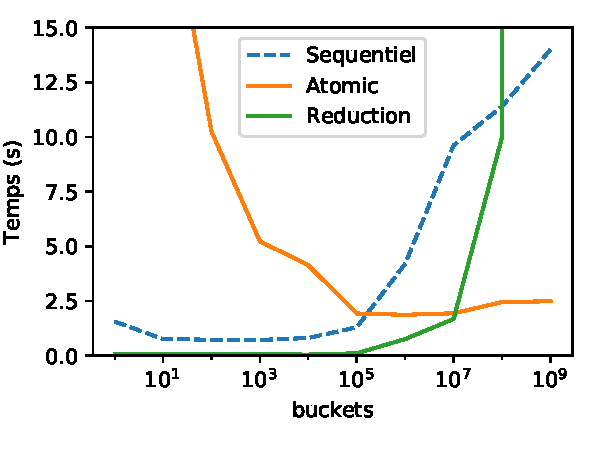
\includegraphics[width=\textwidth]{histogram.pdf}};
    \node at (0, 4) {$N = 10^9$};

    \draw[ultra thick,red,->] (-3, -3.5) node[red,left]{$\times 16$}  -- (-1, -3.5) -- (0.15, -2.4);
  \end{tikzpicture}
\end{frame}


%%%%%%%%%%%%%%%%%%%%%%%%%%%%%%%%%%%%%%%%%%%%%%%%%%%%%%%

\begin{frame}[label=world_of_pain]
  \Huge

  
    \begin{center}

  \scalebox{1.1}{You \textbf{must} follow the rule}

  \pause
  \bigskip
  
  \scalebox{1.1}{Or else...}

  \pause
  \bigskip
  
  \scalebox{1.1}You will be living \\
  In a \textbf{world   of \alert{PAIN}}
\end{center}
\end{frame}

%%%%%%%%%%%%%%%%%%

\begin{frame}
  \frametitle{Don't follow the rules?}

  \centering
  
\includegraphics[width=\textwidth]{goto.png}

  \medskip

  \url{https://xkcd.com/292/}
\end{frame}

%%%%%%%%%%%%%%%%%%%%%%%%%%%%%%%%%%%%%%%%%%%%%%%%%%%

\begin{frame}
  \frametitle{La triste vérité...}

    \begin{columns}[c]
    \begin{column}{.1\textwidth}
      \includegraphics[width=\textwidth]{triste.png}
    \end{column}
    \begin{column}{.9\textwidth}

      
  \begin{itemize}
  \item Barrière $\rightarrow$ attente
  \item Critical $\rightarrow$ séquentialisation
  \item Atomic~  $\rightarrow$ plus lent qu'un accès normal
  \end{itemize}

\end{column}
\end{columns}

\bigskip
  
  Synchronisation $\rightarrow$ limite le passage à l'échelle.

  \bigskip

  $\Longrightarrow$ rôle important de la localité des données.
\end{frame}

%%%%%%%%%%%%%%%%%%%%%%%%%%%%%%%%%%%%%

\begin{frame}[label=guru_switch]
  \begin{exampleblock}{Tout le monde en passe inévitablement par là}
    \begin{itemize}
    \item Bon, mais alors si on évite \texttt{i++}, ça va aller, non ?
    \item J'ai lu dans la doc de mon CPU que les lectures/écritures alignées étaient atomiques ; si on se tient à ça, ça va aller ?
    \end{itemize}
  \end{exampleblock}

  \pause\bigskip
  \begin{alertblock}{Crise d'adolescence}
    Laissons tomber la règle d'or.
  \end{alertblock}

  \pause\bigskip
  
  \begin{tikzpicture}
    \node (switch) {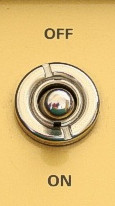
\includegraphics[width=2cm]{switch.jpg}};
    \node[above right=-10mm and 0mm of switch, font={\Large\bfseries}] {Safety};
    \node[below right=-10mm and 0mm of switch, text=red, font={\Large\bfseries}] {World of PAIN};
    \node[left=of switch, font={\large}] (label) {Guru switch};
    \draw (label) edge[->] (switch);
  \end{tikzpicture}
  
\end{frame}    

%%%%%%%%%%%%%%%%%%%%%%%%%%%%%%%%%%%%%

\begin{frame}[fragile, label=peterson_code]
  \begin{block}{Le \emph{Peterson Lock} (1981)}
\begin{minted}{C}
bool flag[2];
int turn;

void lock()
{
    int i = omp_get_thread_num();
    flag[i] = true;                      // I'm interested
    turn   = 1 - i;                      // you go first
    while (turn != i && flag[1-i]) {};   // wait 'til he's not interested
}                                        //    or its my turn

void unlock() 
{
    int i = omp_get_thread_num();
    flag[i] = false;                     // I'm not interested
}
\end{minted}
\end{block}

\begin{alertblock}{CLAIMS}
  \begin{itemize}
  \item Exclusion mutuelle
  \item Pas de \emph{deadlock}
  \item Starvation-free
  \end{itemize}
\end{alertblock}
\end{frame}

%%%%%%%%%%%%%%%%%%%%%%%%%%%%%%%%%%%%%%%%%%

\begin{frame}[label=peterson_demo]
  \frametitle{\emph{Peterson Lock}}

  \centering \Huge \bfseries LIVE DEMO
\end{frame}

%%%%%%%%%%%%%%%%%%%%%%%%%%%%%%%%%%%%%%%%%%

\begin{frame}[label=peterson_report1, fragile]

  \begin{block}{Guru problem \#1: \bfseries Trahison du compilateur}
    \begin{itemize}
      \item On avait :
    \begin{minted}{C}
    turn = 1 - i;                      // you go first
    while (turn != i && flag[1-i]) {}; // wait
\end{minted}

\item L'optimiseur \og sait\fg{} que \texttt{turn != i}
\item Donc ceci devient :
  \begin{minted}{C}
void lock()
{
    int i = omp_get_thread_num();
    flag[i] = true;                      // I'm interested
    while (flag[1-i]) {};                // wait
}
\end{minted}
\item Les deux threads appellent \texttt{lock()} en même temps...
\item ... \texttt{flag[0] == flag[1] == true} ...
\item Deadlock.
\end{itemize}
\end{block}
\end{frame}

%%%%%%%%%%%%%%%%%%%%%%%%%%%%%%%%%%%%%%%%%%

\begin{frame}[label=peterson_report2, fragile]

  \begin{block}{Guru problem \#2: \bfseries ???}
    \begin{itemize}
    \item Défaut d'exclusion mutuelle
    \item Les deux threads pénètrent simultanément dans la section critique
    \item Comment est-ce possible ?
    \end{itemize}
  \end{block}
\end{frame}

%%%%%%%%%%%%%%%%%%%%%%%%%%%%%%%%%%%%


\begin{frame}[label=order]
  \frametitle{Relations d'ordre sur les accès à la mémoire}
  
  \setlength{\leftmargini}{-2mm}
  \begin{itemize}
    \item Accès mémoire :  
      \begin{align*}
        W_i(x)a &: \text{$T_i$ écrit la valeur $a$ dans la variable $x$} \\
        R_i(x)b &: \text{$T_i$ lit la variable $x$ et la valeur $b$}
      \end{align*}

    \item \og \emph{Program Order}\fg{} :
      \begin{align*}
        x \po y &: \text{le code demande qu'on fasse $x$ d'abord et $y$ après}
      \end{align*}

    \item \og \emph{Extended Communication Order}\fg{} :
      \[
      \begin{array}{rcll}
        W(x)a &\rf &R(x)a &: \text{la lecture renvoie la valeur écrite}\\
        W(x)a &\mo& W(x)b &: \text{l'écriture de $a$ a lieu avant celle de $b$}\\
        R(x)a &\rb& W(x)b &: \text{la lecture a lieu avant l'écriture}\\
              &   &       & \quad\text{par définition, } \rb = (\rf)^{-1} ; \mo
      \end{array}
    \]
  \end{itemize}

    \begin{overlayarea}{\textwidth}{2.5cm}
\begin{onlyenv}<2>   
\begin{center}
\begin{tikzpicture}[>=latex]
\foreach \i in {0,1}
  \draw[thick, ->] (0,1-\i) node[left] {$T_\i$} -- +(8,0);

\foreach \i / \j in {1/1, 2/0, 3/1}
  \draw[thick] (2*\i,\j) +(0,0.125) -- +(0, -0.125);

\node[above=1mm] at (6,1) (rx) {$R_0(x)b$};
\node[above=1mm] at (4,0) (w1x) {$W_1(x)b$};
\node[above=1mm] at (2,1) (w0x) {$W_0(x)a$};

\draw[Green,->] (w1x) |- node[above,font=\ttfamily] {rf} (rx);
\draw[orange,->] (w0x) -- node[below,font=\ttfamily] {mo} (w1x);

\end{tikzpicture}
\end{center}
\end{onlyenv}

% \begin{theorem}<3>
%   Sequential Consistency $\Longleftrightarrow$ pas de cycles avec $\po \cup \rf \cup \co \cup \fr$.
% \end{theorem}
\end{overlayarea}
\end{frame}

%%%%%%%%%%%%%%%%%%%%%%%%%%%%%%%%%%%%

\begin{frame}[label=order2]
  \frametitle{Relations d'ordre entre accès à la mémoire}
 
   { \small
      \[
      \begin{array}{rcll}
        W(x)a &\rf &R(x)a &: \text{la lecture renvoie la valeur écrite}\\
        W(x)a &\mo& W(x)b &: \text{l'écriture de $a$ a lieu avant celle de $b$}\\
        R(x)a &\rb& W(x)b &: \text{la lecture a lieu avant l'écriture} \\
              &   &       & \quad\text{par définition, } \rb = (\rf)^{-1} ; \mo
      \end{array}
    \]
}
    \bigskip

    \begin{block}{Intuition}
    \begin{itemize}
    \item En principe, $\rf, \mo, \rb$ ne peuvent pas \og contredire\fg{} $\po$
    \item On ne lit pas de valeur \og périmée\fg{} ($\rb$ à l'envers)
    \item<2-> Pas de lecture \og depuis le futur\fg{} ($\rf$ à l'envers)
    \end{itemize}
  \end{block}

  \begin{overlayarea}{\textwidth}{3cm}
  \begin{center}
    \begin{onlyenv}<1>
    \begin{tikzpicture}[>=latex, every node/.style={inner sep=1pt}]
      \draw[thick, ->] (1, 0) node[left] {$T_0$} -- +(8,0);
      
      \foreach \i in {1, 2, 3}
      \draw[thick] (2.5*\i, 0) +(0,0.125) -- +(0, -0.125);
      
      \node[above=2mm] at (2.5,0) (w0x) {$W_0(x)a$};
      \node[above=2mm] at (5,0) (w1x) {$W_0(x)b$};
      \node[above=2mm] at (7.5,0) (rx) {$R_0(x)a$};

      
      \draw[orange,->] (w0x) edge node[above,font=\ttfamily] {mo} (w1x);
      \draw[Green,->] (w0x) edge[bend right] node[below,font=\ttfamily] {rf} (rx);
      \draw[Purple,->] (rx) edge node[above,font=\ttfamily] {rb} (w1x);
    \end{tikzpicture}
  \end{onlyenv}

  \begin{onlyenv}<2>
    \begin{tikzpicture}[>=latex]
      \draw[thick, ->] (1, 0) node[left] {$T_0$} -- +(8,0);
      
      \foreach \i in {1, 2, 3}
      \draw[thick] (2.5*\i, 0) +(0,0.125) -- +(0, -0.125);
      
      \node[above=1mm] at (2.5,0) (w1x) {$W_0(x)a$};
      \node[above=1mm] at (5,0) (rx) {$R_0(x)b$};
      \node[above=1mm] at (7.5,0) (w0x) {$W_0(x)b$};
      
      \draw[Green,->] (w0x) edge[] node[above,font=\ttfamily] {rf} (rx);
    \end{tikzpicture}
  \end{onlyenv}
\end{center}
\end{overlayarea}
\end{frame}

%%%%%%%%%%%%%%%%%%%%%%%%%%%%%%%%%%%%

\begin{frame}[label=order2]
  \frametitle{Relations d'ordre entre accès à la mémoire} 
   { \small
      \[
      \begin{array}{rcll}
        W(x)a &\rf &R(x)a &: \text{la lecture renvoie la valeur écrite}\\
        W(x)a &\mo& W(x)b &: \text{l'écriture de $a$ a lieu avant celle de $b$}\\
        R(x)a &\rb& W(x)b &: \text{la lecture a lieu avant l'écriture} \\
              &   &       & \quad\text{par définition, } \rb = (\rf)^{-1} ; \mo
      \end{array}
    \]
}
    \medskip

    En séquentiel : $\rf \subseteq \po$, $\mo \subseteq \po$ et $\rb \subseteq \po$

    \medskip
    
    \begin{alertblock}{C'est faux en parallèle}
\begin{center}
\begin{tikzpicture}[>=latex,scale=0.9]
\foreach \i in {0,1}
  \draw[thick, ->] (0,1-\i) node[left] {$T_\i$} -- +(8,0);

\foreach \i / \j in {1/1, 2/0, 3/1}
  \draw[thick] (2*\i,\j) +(0,0.125) -- +(0, -0.125);

\node[above=1mm] at (6,1) (rx) {$R_0(x)b$};
\node[above=1mm] at (4,0) (w1x) {$W_1(x)b$};
\node[above=1mm] at (2,1) (w0x) {$W_0(x)a$};

\draw[Green,->] (w1x) |- node[above,font=\ttfamily] {rf} (rx);
\draw[orange,->] (w0x) -- node[below,font=\ttfamily] {mo} (w1x);
\end{tikzpicture}
\end{center}
\end{alertblock}    
\end{frame}

%%%%%%%%%%%%%%%%%%%%%%%%%%%%%%%%%%%%%%%%%%%%%%%%%%

\section{La Sequential Consistency}

\begin{frame}[label=seq_cst]
  \frametitle{La \emph{Sequential Consistency}}

  \begin{exampleblock}{Intuition}
    Tout se passe comme si les accès mémoires étaient exécutées
    \emph{séquentiellement} (dans un ordre qu'on ne connaît pas forcément).
  \end{exampleblock}

  \pause
  
  \begin{definition}[Sequential Consistency]
    Un système parallèle est \alert{séquentiellement consistant} si, pour
    chacune des exécutions possibles des threads auxquelles il peut aboutir, on
    peut construire un \alert{historique} $H$ :
    \begin{itemize}
    \item séquence totalement ordonnée
    \item contient une et une seule fois chaque accès mémoire
    \item compatible avec le code des threads (respecte $\po$)
    \item lecture de la dernière valeur écrite
    \end{itemize}
  \end{definition}

  \small
  
\begin{theorem}
   Sequential Consistency $\Longleftrightarrow$ pas de cycles avec $\po \cup \rf \cup \mo \cup \rb$.
 \end{theorem}
\end{frame}


%%%%%%%%%%%%%%%%%%%%%%%%%%%%%%%%%%%%%%%%%%%%%%%%%%%%%%

\againframe{peterson_code}

%%%%%%%%%%%%%%%%%%%%%%%%%%%%%%%%%%%

\begin{frame}[label=peterson_thm]
  \frametitle{Correction du \emph{Peterson Lock}}

  \begin{exampleblock}{\emph{Sequential Consistency}}
    Tout se passe comme si les accès mémoires étaient exécutées
    \emph{séquentiellement} (dans un ordre qu'on ne connaît pas forcément).
  \end{exampleblock}

  \begin{theorem}
    Si la mémoire est séquentiellement consistante, alors le \emph{Peterson
      lock} garantit l'exclusion mutuelle.
  \end{theorem}

  \bigskip

  Preuve : ...
\end{frame}

%%%%%%%%%%%%%%%%%%%%%%%%%%%%%%%%%%%%

\begin{frame}[label=peterson_proof]
  \setlength{\leftmargini}{-3mm}
  \small
  \begin{itemize}
  \item Absurde : $T_0$ et $T_1$ appellent \texttt{lock()}, entrent dans la section critique.
  \item État initial : \mintinline{C}{flag[0] = false; flag[1] = false;}
  \item D'après le code :
  \footnotesize
  \begin{align*}
    T_0 &: W_0(\mintinline{C}{flag[0]}) \mintinline{C}{true} \po  W_0(\mintinline{C}{turn}) 1 \po  R_0(\mintinline{C}{turn})? \po R_0(\mintinline{C}{flag[1]})? \po CS_0 \\
    T_1 &: W_1(\mintinline{C}{flag[1]}) \mintinline{C}{true} \po  W_1(\mintinline{C}{turn}) 0 \po R_1(\mintinline{C}{turn})? \po R_1(\mintinline{C}{flag[0]})? \po CS_1
  \end{align*}
\item \small Supposons que $T_0$ écrive \texttt{turn} en dernier :
  \footnotesize
  \[
    W_1(\mintinline{C}{turn}) 0 \mo W_0(\mintinline{C}{turn}) 1.
  \]
\item \small $T_0$ sort de la boucle, et $\texttt{turn == 1}$, donc forcément :
  \footnotesize
  \[
    W_0(\mintinline{C}{turn}) 1 \po  R_0(\mintinline{C}{turn}) 1 \po R_0(\mintinline{C}{flag[1]}) \mintinline{C}{false}.
  \]
\item \small Si on met tout ceci bout-à-bout :
  \begin{tikzpicture}[every node/.style={font=\footnotesize, inner sep=1pt}]
    \path[use as bounding box] (0, -0.75) rectangle (11, 1.5);
    \node[anchor=west] at (-0.15, 1) (Winit) { $W_{init}(\mintinline{C}{flag[1]}) \mintinline{C}{false}$ };
    \node[anchor=west] at (0, 0) (Wflag) { $W_1(\mintinline{C}{flag[1]}) \mintinline{C}{true}$ };
    %\po
    \node[anchor=west] at (3.25, 0) (Wturn1) { $W_1(\mintinline{C}{turn}) 0$ };
    % \co
    \node[anchor=west] at (6, 0) (Wturn0) { $W_0(\mintinline{C}{turn}) 1$};
    % \po
    \node[anchor=west] at (8.75, 0) (Rflag) { $R_0(\mintinline{C}{flag[1]}) \mintinline{C}{false}$};

    \draw[orange] (Winit) edge[->] node[right] {$\scriptstyle \texttt{mo}$} (Wflag);
    \draw (Wflag) edge[->] node[above] {$\scriptstyle \texttt{po}$} (Wturn1);
    \draw[orange] (Wturn1) edge[->] node[above] {$\scriptstyle \texttt{mo}$} (Wturn0);
    \draw (Wturn0) edge[->] node[above] {$\scriptstyle \texttt{po}$} (Rflag);

    \draw[Green] (Winit.east) edge[out=0,in=160,->] node[above] {$\scriptstyle \texttt{rf}$} (Rflag.north west);

    \draw[Purple,->] (Rflag.south) -- +(0, -0.5) -| node[below,near start] {$\scriptstyle \texttt{rb}$} (Wflag.south);
  \end{tikzpicture}

\item \small Cycle $\Rightarrow$ non-SC $\Rightarrow$ Contradiction !
\end{itemize}
\end{frame}

%%%%%%%%%%%%%%%%%%%%%%%%%%%%%%%%%%%%%%%%%%%%%%%%%%%%%%%%%

\begin{frame}[label=peterson_report1, fragile]

  \begin{block}{Guru problem \#2: \bfseries défaut de \emph{sequential consistency}}

    \begin{itemize}
    \item Preuve : sequential consistency $\Rightarrow$ mutual exclusion
    \item Observation : \sout{mutual exclusion}
    \item Conséquence : 
    \end{itemize}
    
    \begin{columns}[c]
    \begin{column}{.1\textwidth}
      \includegraphics[width=\textwidth]{triste.png}
    \end{column}
    \begin{column}{.9\textwidth}
      \begin{itemize}
      \item Mon laptop n'est pas séquentiellement consistent...
        \pause
      \item Le tien ne l'est pas non plus !
      \end{itemize}
    \end{column}
  \end{columns}

\end{block}
\end{frame}

%%%%%%%%%%%%%%%%%%%%%%%%%%%%%%%%%%%%%%%%%%

%%%%%%%%%%%%%%%%%%%%%%%%%%%%%%%%%%%%%%%%%%%%% 

\begin{frame}[fragile, label=cpu_not_cs]
  \frametitle{Les CPU ne sont pas séquentiellement consistents !}
  \framesubtitle{La \emph{Sequential Consistency} est coûteuse}
  \begin{center}
    \begin{tikzpicture}
      \path[red,dotted,use as bounding box] (-2,-5) rectangle (8,2);
      % "RAM"
      \begin{scope}[yshift=1.75cm, every node/.style={anchor=base}]
        \draw[thick] (1, -0.2) rectangle (5, 0.4);
        \node<1-2> at (2, 0) {$x = 0$};
        \node<1-2> at (4, 0) {$y = 0$};
        \node<3-> at (2, 0) {$x = 1$};
        \node<3-> at (4, 0) {$y = 1$};
      \end{scope}

      \node (CPU1) at (0, 0) {
\includegraphics[width=2cm]{cpu_clipart.png}};
      \node<1-2>[draw,anchor=east] at (-1.5, 0) {$w = 0$};
      \node<3->[draw,anchor=east] at (-1.5, 0) {$w = ?$};
      
      \node (CPU2) at (6, 0) {
\includegraphics[width=2cm]{cpu_clipart.png}};
      \node<1-2>[draw,anchor=west] at (7.5, 0) {$z = 0$};
      \node<3->[draw,anchor=west] at (7.5, 0) {$z = ?$};

      \draw[very thick] (CPU1) edge[<->] node[above] {temps $\geq \tau$} (CPU2);
      \draw[thick,<->] (CPU1) |- (0.9, 1.85);
      \draw[thick,<->] (CPU2) |- (5.1, 1.85);

    \node<2->[align=center] at (0, -1.5) {\mintinline[fontsize=\normalsize]{C}{x = 1;} \\ \mintinline[fontsize=\normalsize]{C}{w = y;}};
    \node<2->[align=center] at (6, -1.5) {\mintinline[fontsize=\normalsize]{C}{y = 1;} \\ \mintinline[fontsize=\normalsize]{C}{z = x};};

    \node<3> at (3, -2.5) {\emph{Sequential Consistency} $\Rightarrow (w,z) \neq (0, 0)$};
    
    % preuve sous SC.
    \begin{onlyenv}<4>
    \begin{scope}[>=latex, scale=0.75, yshift=-6.5cm, xshift=-2cm, every node/.style={inner sep=1pt}]
      \foreach \i in {0,1}
      \draw[thick, ->] (0,1-\i) node[left] {$T_\i$} -- +(12,0);
      
      \foreach \i / \j in {6/1, 10/1, 6/0, 10/0}
      \draw[thick] (\i,\j) +(0,0.125) -- +(0, -0.125);

      \node[] at (1, 3) (initx) {$W_{init}(x)0$};
      \node[] at (1, 2) (inity) {$W_{init}(y)0$};
      
      \node[above=2mm] at (6,1)  (wx) {$W_0(x)1$};
      \node[above=2mm] at (10,1) (ry) {$R_0(y)0$};
      \node[above=2mm] at (6,0)  (wy) {$W_1(y)1$};
      \node[above=2mm] at (10,0) (rx) {$R_1(x)0$};
      \begin{scope}[every node/.style={font=\ttfamily\small}]
      \draw[Green,->] (inity.north east) to[bend left]  node[above] {rf} (ry);
      \draw[Green,->] (initx.south east) to[bend right] node[below, very near end] {rf} (rx);      
      \draw[orange,->] (inity.east) to node[below, very near start] {mo} (wy.north west);
      \draw[orange,->] (initx.east) to node[above, near end] {mo} (wx.north west);
      \draw[Purple,->] (ry) edge node[above, near start] {rb} (wy);
      \draw[Purple,->] (rx) edge node[below, near start] {rb} (wx);
    \end{scope}
  \end{scope}
  \end{onlyenv}

  % preuve du délai.
  \begin{onlyenv}<5>
    \begin{scope}[xshift=3cm,yshift=-2.5cm]
      \node at (0, 0) {$r$ : temps min. pour faire une lecture};
      \node at (0, -0.5) {$w$ : temps min. pour faire une écriture};

      \node[text=red] at (0, -1.5) {\emph{Sequential Consistency} $\Longrightarrow$ $r + w \geq \tau$};
      \node[font=\footnotesize] at (0, -2) {L'un doit bien lire l'écriture de l'autre...};
    \end{scope}
    \draw[very thick, red, <->] (1.15, -0.5)  -- node[below] {$w$} (3, -0.5);
    \draw[very thick, red, <->] (4.85, -0.5) -- node[below] {$r$} (4, -0.5);
  \end{onlyenv}
\end{tikzpicture}
\end{center}
\end{frame}

%%%%%%%%%%%%%%%%%%%%%%%%%%%%%%%%%%%%%%%%%%%%%%%%%%%%%%%%%

\begin{frame}[label=tso]
  \frametitle{Le \emph{Store Buffering}}
  
  \centering
  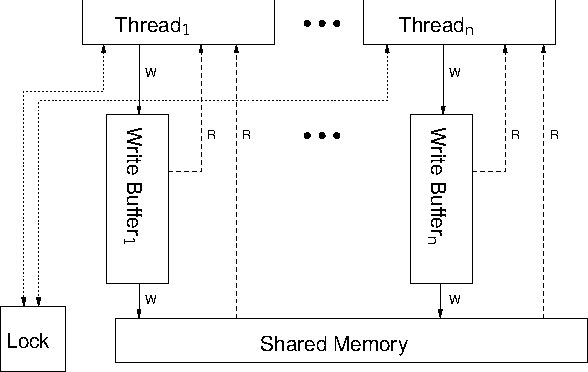
\includegraphics[width=\textwidth]{tso}

  \medskip
  
  \scriptsize (image~:~A Tutorial
    Introduction to the ARM and POWER Relaxed Memory Models)
\end{frame}

%%%%%

\begin{frame}[label=tso]
  \frametitle{Architectures avec \emph{Total Store Ordering}}
  \framesubtitle{x86 et SPARC}
  
  \begin{block}{Chaque thread \alert{matériel} possède un \textbf{Store Buffer}}
    \begin{itemize}
    \item Mes écritures sont placées en attente dans mon \emph{Store Buffer}
    \item C'est une file (on ne double pas !)
    \item Je \emph{vois} mes écritures tout de suite
    \item Mon \emph{Store Buffer} \alert{sera} \og vidangé\fg{} vers la mémoire... à terme
    \item À ce moment-là :
      \begin{itemize}
      \item  \emph{Tous les autres threads} voient mes écritures.
      \item Ils les voient dans le même ordre.
      \end{itemize}
    \end{itemize}
  \end{block}
\end{frame}

%%%%%%%%%%%%%%%%%%%%%%%%%%%%%%%%%%%%%%%%%%%%%%%%%%%%%%%% 

\begin{frame}[fragile, label=peterson_code_tso]
  \frametitle{Échec du \emph{Peterson Lock} en présence de \emph{Store Buffering}}

  \begin{columns}
    \begin{column}{0.5\textwidth}
      \begin{block}{Le \og \emph{Peterson Lock}\fg{}}
\begin{minted}{C}
bool flag[2];
int victim;

void lock() 
{
    int i = omp_get_thread_num();
    flag[i] = true;
    turn = 1 - i;
    while (turn != i && flag[1-i])
        {};
}
\end{minted}
      \end{block}
    \end{column}  
    \begin{column}{0.5\textwidth}
      \begin{tikzpicture}[scale=0.5]
        \path[red,dotted,use as bounding box] (-2.5, -10.5) rectangle (9, 0);
        \draw (-2.5, -10.5) rectangle (8.5, -9.5);

        \draw[dashed] (-2.5, -2.5) rectangle +(5, -5);
        \draw[dashed] (3.5, -2.5) rectangle +(5, -5);
        
        \node<1-3> at (0, -10) (flag0) {\mintinline{C}{flag[0] = false}};
        \node<1-3> at (6, -10) (flag1) {\mintinline{C}{flag[1] = false}};
        \node<4> at (0, -10) (flag0) {\mintinline{C}{flag[0] = true}};
        \node<4> at (6, -10) (flag1) {\mintinline{C}{flag[1] = true}};

        
        \node at (0, 0) (T0) {
\includegraphics[width=1cm]{cpu_clipart.png}};
        \node at (6, 0) (T1) {
\includegraphics[width=1cm]{cpu_clipart.png}};

        \node[below=of T0] (w0v) {\mintinline{C}{turn = 1}};
        \node[below=of w0v] (w0f) {\mintinline{C}{flag[0] = true}};

        \node[below=of T1] (w1v) {\mintinline{C}{turn = 0}};
        \node[below=of w1v] (w1f) {\mintinline{C}{flag[1] = true}};

        \draw[->] (T0) edge (w0v);
        \draw[->] (w0v) edge (w0f);

        \draw[->] (T1) edge (w1v);
        \draw[->] (w1v) edge (w1f);

        \draw<4>[->] (w0f) edge (flag0);
        \draw<4>[->] (w1f) edge (flag1);

        
        \draw<2>[thick,Green] (w0v.north west) edge[bend left,->] node[above,sloped,font=\ttfamily] {rf} (T0);
        \draw<3>[thick,Green] (flag1) edge[bend right,->] node[very near end, below,sloped,font=\ttfamily] {rf} (T0);
        \draw<2>[thick,Green] (w1v.north east) edge[bend right,->] node[above,sloped,font=\ttfamily] {rf} (T1);
        \draw<3>[thick,Green] (flag0) edge[bend left,->] node[very near end, below,sloped,font=\ttfamily] {rf} (T1);

      \end{tikzpicture}
    \end{column}
  \end{columns}
\end{frame}

%%%%%%%%%%%%%%%%%%%%%%%%%%%%%%%%%%%%%%%%%%%%%%%%%%%%%%%

%%%%%

\begin{frame}[fragile, label=tso_mp]
  \frametitle{Le \emph{Message Passing} }
  
  \begin{columns}
    \begin{column}{0.5\textwidth}
      \begin{block}{\emph{Producer}}
\begin{minted}{C}
void produce(void *payload)
{          
    msg = payload;
    flag = true;
}
\end{minted}
      \end{block}
    \end{column}  
    \begin{column}{0.5\textwidth}
      \begin{block}{\emph{Receiver}}
\begin{minted}{C}
void * receive()
{  
    while (!flag) {}; // wait
    return msg;
}
\end{minted}
      \end{block}
    \end{column}
  \end{columns}

  \begin{overlayarea}{\textwidth}{1cm}
    \begin{onlyenv}<2>
      \begin{columns}[c]
        \begin{column}{.1\textwidth}
          \vspace{1mm}
          
\includegraphics[width=\textwidth]{Content.png}
        \end{column}

        \begin{column}{.9\textwidth}
          \begin{itemize}        \small
          \item Fonctionne en cas de  \emph{Total Store Ordering}
          \item x86, SPARC, \dots
          \end{itemize}
        \end{column}
      \end{columns}
    \end{onlyenv}
    
    \begin{onlyenv}<3->  
      \begin{columns}[c]
        \begin{column}{.1\textwidth}
          \vspace{3mm}
          \includegraphics[width=\textwidth]{triste.png}
        \end{column}
        
        \begin{column}{.9\textwidth}
          \begin{itemize}        \small
          \item Ne fonctionne pas sur ARM, POWER, ...
          \item Les threads ne \emph{voient} pas les écritures dans le même ordre !
          \end{itemize}
        \end{column}
      \end{columns}  
    \end{onlyenv}
  \end{overlayarea}
  
  \begin{uncoverenv}<4>  
    \begin{center}
      \begin{tikzpicture}[>=latex,scale=0.85,every node/.style={font=\small,inner sep=1pt}]
        \path[use as bounding box] (0, 0) rectangle +(12, 3.5);
        \foreach \i in {0,1}
        \draw[thick, ->] (0,1-\i) node[left] {$T_\i$} -- +(12,0);
        
        \foreach \i / \j in {6/1, 10/1, 6/0, 10/0}
        \draw[thick] (\i,\j) +(0,0.125) -- +(0, -0.125);
        
        \node[above] at (2,2) (initx) {$W_{init}(msg)0$};
%        \node[above] at (1,1) (inity) {$W_{init}(flag)0$};
        
        
        \node[above=1mm] at (6,1)  (wx) {$W_0(msg)1$};
        \node[above=1mm] at (10,1) (wy) {$W_0(flag)1$};
        \node[above=1mm] at (6,0)  (ry) {$R_1(flag)1$};
        \node[above=1mm] at (10,0) (rx) {$R_1(msg)0$};
        \begin{scope}[every node/.style={font={\small\ttfamily}}]
        \draw[thick,Green,->] (initx) edge[bend right]  node[below, very near end] {rf} (rx);
        \draw[thick,Green,->] (wy) edge  node[above, near start] {rf} (ry);        
        \draw[thick,orange,->] (initx.east) to  node[above] {mo} (wx.west);
        \draw[thick,purple,->] (rx) edge  node[below, near start] {rb} (wx);
      \end{scope}
    \end{tikzpicture}
    \end{center}
  \end{uncoverenv}
\end{frame}

%%%%%%%%%%%%%%%%%%%%%%%%%%%%%%%%%%%%%%%%%%%%%%%%%%%%%% 

%%%%%%%%%%%%%%%%%%%%%%%%%%%%%%%%%%%%%%%%%%%%%%%%%%%%%%%

\begin{frame}[label=omp_memory_model]
\frametitle{Modèle mémoire dans OpenMP}

% \normalsize
% \setlength{\leftmargini}{0mm}
% \begin{itemize}
% \item Les processeurs ont des modèles mémoires \alert{relachés} (\og \textit{relaxed}\fg{})
%   \begin{itemize}
%   \item Question de performance
%   \end{itemize}
%   \item[$\Rightarrow$] OpenMP s'adapte
% \end{itemize}

Bien sûr les threads ont accès à la mémoire partagée, mais...


\begin{alertblock}{Un thread a une \textbf{vue temporaire privée} de la mémoire}
  \begin{itemize}
  \item Pas forcément synchronisée en permanence.

  \item Une lecture \textbf{peut} provenir de la vue temporaire privée.
    
  \item Une écriture \textbf{peut} rester dans la vue temporaire privée.

  \item Synchronisation (implicite) lors de:
    \begin{itemize}
    \item \texttt{\#pragma omp barrier}
    \item sortie de \texttt{\#pragma omp for/sections/single}
    \item entrée/sortie de \texttt{\#pragma omp parallel/critical/atomic}
    \item \emph{Task Scheduling Points}
    \end{itemize}

  \item Synchronisation (explicite) avec \texttt{\#pragma omp flush}
  \end{itemize}
\end{alertblock}

  \begin{exampleblock}{Opérations atomiques (\texttt{\#pragma omp atomic})}
    \begin{itemize}
    \item Obéissent à la \emph{sequential consistency}
    \end{itemize}
  \end{exampleblock}

\end{frame}

%%%%%%%%%%%%%%%%%%%%%%%

\begin{frame}[label=pram]
  \frametitle{Représentation schématique}
  
  \centering
  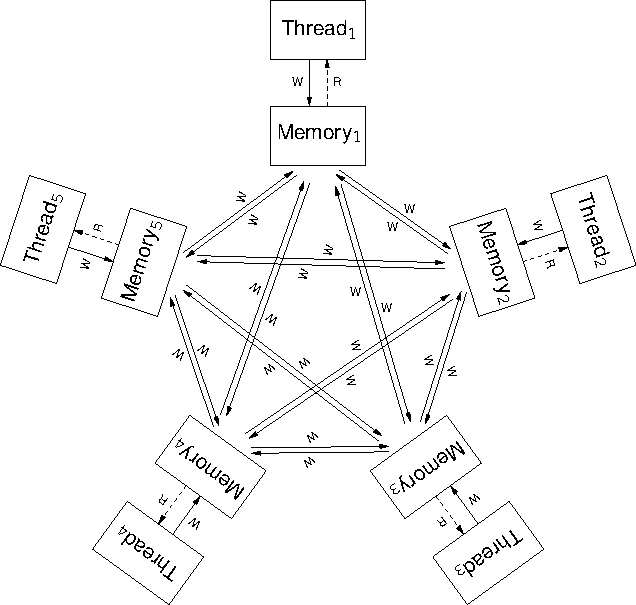
\includegraphics[height=8cm]{pram_archi.pdf}
    \medskip
  
  \scriptsize (image~:~A Tutorial
    Introduction to the ARM and POWER Relaxed Memory Models)

\end{frame}

%%%%%%%%%%%%%%%%%%%%%%%%

\againframe<3>{guru_switch}
\againframe{golden_rule}

%%%%%%%%%%%%%%%%%%%%%%%%%%%%%%%%%%%%

%%%%%%%%%%%%%%%%%%%%%%%%%%%%%%%%%%%%%%%%%%%%%%%%%%%%%%%%

\section{Modifier les algos pour éviter les conflits}

%%%%%%%%%%%%%%%%%%%%%%%%%%%%%%%%%%%%%%%%%%%%%%%%%%%%%%%%

\section{Modifier les algos pour éviter les conflits}


\subsection{Bucket Sort}

%%%%%%%%%%%%%%%%%%%%%%%%%%%%%%%%%%
      \pgfmathdeclarerandomlist{MyRandomColors}{{pink}{red}{orange}{yellow}{green}{cyan}{blue}{magenta}{violet}{lightgray}{darkgray}}

      
\begin{frame}[fragile,label=radix]
  \frametitle{Exemple : Bucket Sort}

%int C[256];
%for (int i = 0; i < 256; i++)
%    C[i] = 0;

    \begin{columns}[c]
    \begin{column}{.4\textwidth}

\begin{minted}{C}
// Initialization
for (int i = 0; i < M; i++) {
    C[i] = 0;
}

// Histogram
for (int i = 0; i < N; i++) {
    int bucket = f(A[i]);
    C[bucket]++;
}

// Prefix-sum
int s = 0;
for (int i = 0; i < M; i++) {
    P[i] = s;
    s += C[i];
}

// Dispatch
for (int i = 0; i < N; i++) {
    int bucket = f(A[i]);
    B[P[bucket]] = A[i];
    P[bucket]++;
}
\end{minted}
    \end{column}
    \begin{column}{.6\textwidth}


      \begin{tikzpicture}[scale=0.25, >={To[sep]}]
        \path[red,dotted,use as bounding box] (-1, 0) rectangle +(26, 32);
        
        % état initial aléatoire
        \pgfmathsetseed{57}
        \foreach \i in {0, 1, ..., 31} {
          \pgfmathrandomitem{\RandomColor}{MyRandomColors} 
          \fill[fill=\RandomColor] (0, \i) rectangle +(3, 1);
        }
        \draw[thick] (0, 0) rectangle +(9, 32);
        \draw[thick] (3, 0) -- +(0, 32);
        \foreach \i in {1, ..., 31} {
          \draw (0, \i) -- +(9, 0);
        }
        \foreach \i / \l in {0/3, 1/0, 2/7, 3/1, 4/10, 5/2, 6/5, 7/2, 8/10, 9/5,
          10/2, 11/3, 12/8, 13/7, 14/9, 15/10, 16/3, 17/6, 18/4, 19/6,
          20/10, 21/0, 22/5, 23/3, 24/5, 25/9, 26/5, 27/7, 28/8, 29/9,
          30/8, 31/5} {
%          \node[font=\tiny] at (-1, 31.5-\i) {\i};
          \node[font=\tiny] at (4, 31.5-\i) {\l};
        }
        
        % côté droit : trié
        \begin{scope}[xshift=16cm]
          % situation finale supposée
          \begin{onlyenv}<1-3>
          \fill[fill=pink] (0, 30) rectangle +(3, 2);
          \fill[fill=magenta] (0, 29) rectangle +(3, 1);
          \fill[fill=violet] (0, 26) rectangle +(3, 3);
          \fill[fill=blue] (0, 22) rectangle +(3, 4);
          \fill[fill=cyan] (0, 21) rectangle +(3, 1);
          \fill[fill=green] (0, 15) rectangle +(3, 6);
          \fill[fill=yellow] (0, 13) rectangle +(3, 2);
          \fill[fill=orange] (0, 10) rectangle +(3, 3);
          \fill[fill=red] (0, 7) rectangle +(3, 3);
          \fill[fill=lightgray] (0, 4) rectangle +(3, 3);
          \fill[fill=darkgray] (0, 0) rectangle +(3, 4);
        \end{onlyenv}

        % \begin{onlyenv}<4->
        %     \fill[very nearly transparent, fill=pink] (0, 30) rectangle +(3, 2);
        %     \fill[very nearly transparent, fill=magenta] (0, 29) rectangle +(3, 1);
        %     \fill[very nearly transparent, fill=violet] (0, 26) rectangle +(3, 3);
        %     \fill[very nearly transparent, fill=blue] (0, 22) rectangle +(3, 4);
        %     \fill[very nearly transparent, fill=cyan] (0, 21) rectangle +(3, 1);
        %     \fill[very nearly transparent, fill=green] (0, 15) rectangle +(3, 6);
        %     \fill[very nearly transparent, fill=yellow] (0, 13) rectangle +(3, 2);
        %     \fill[very nearly transparent, fill=orange] (0, 10) rectangle +(3, 3);
        %     \fill[very nearly transparent, fill=red] (0, 7) rectangle +(3, 3);
        %     \fill[very nearly transparent, fill=lightgray] (0, 4) rectangle +(3, 3);
        %     \fill[very nearly transparent, fill=darkgray] (0, 0) rectangle +(3, 4);
        %   \end{onlyenv}

          % items qui arrivent en cours de route
          \fill<5->[fill=blue] (0, 25) rectangle +(3, 1);
          \fill<9->[fill=pink] (0, 31) rectangle +(3, 1);
          \fill<11->[fill=orange] (0, 12) rectangle +(3, 1);
          
          % cadre
          \draw[thick] (0, 0) rectangle +(9, 32);
          \draw[thick] (3, 0) -- +(0, 32);
          \foreach \i in {1, ..., 31} {
            \draw (0, \i) -- +(9, 0);
          }
      \end{scope}

      % taille des buckets
      \begin{onlyenv}<2>
        \draw[<->] (15, 30) -- node[left] {$C[0]$} +(0, 2);
        \draw[<->] (15, 26) -- node[left] {$C[2]$} +(0, 3);
        \draw[<->] (15, 22) -- node[left] {$C[3]$} +(0, 4);
        \draw[<->] (15, 15) -- node[left] {$C[5]$} +(0, 6);
        \draw[<->] (15, 13) -- node[left] {$C[6]$} +(0, 2);
        \draw[<->] (15, 10) -- node[left] {$C[7]$} +(0, 3);
        \draw[<->] (15, 7) -- node[left] {$C[8]$} +(0, 3);
        \draw[<->] (15, 4) -- node[left] {$C[9]$} +(0, 3);
        \draw[<->] (15, 0) -- node[left] {$C[10]$} +(0, 4);
      \end{onlyenv}

      % pointeurs initiaux sur les buckets
      \begin{onlyenv}<3->
        \draw<-8>[->] (15, 31.5) node[left] {$P[0]$} -- (16, 31.5);
        \draw[->] (15, 28.5) node[left] {$P[2]$} -- (16, 28.5);
        \draw<-5>[->] (15, 25.5) node[left] {$P[3]$} -- +(1, 0);
        \draw[->] (15, 20.5) node[left] {$P[5]$} -- (16, 20.5);
        \draw[->] (15, 14.5) node[left] {$P[6]$} -- (16, 14.5);
        \draw<-11>[->] (15, 12.5) node[left] {$P[7]$} -- (16, 12.5);
        \draw[->] (15, 9.5)  node[left] {$P[8]$} -- (16,  9.5);
        \draw[->] (15, 6.5)  node[left] {$P[9]$} -- (16,  6.5);
        \draw[->] (15, 3.5)  node[left] {$P[10]$}-- (16,  3.5);
      \end{onlyenv}
    
      % pointeurs modifiés
      \draw<6->[->] (15, 24.5) node[left] {$P[3]$} -- +(1, 0);
      \draw<9->[->] (15, 30.5) node[left] {$P[0]$} -- +(1, 0);
      \draw<12->[->] (15, 11.5) node[left] {$P[7]$} -- +(1, 0);
      
      % flèches de progression à gauche
      \draw<4-5>[thick,->] (-2, 31.5) -- +(2, 0);
      \draw<7-8>[thick,->] (-2, 30.5) -- +(2, 0);
      \draw<10-11>[thick,->] (-2, 29.5) -- +(2, 0);

      \draw<5>[->] (9, 31.5) -- (10, 30.5) -- (10, 27) -- (14, 27) -- (16, 26);
      \draw<8>[->] (9, 30.5) -- (14, 30.5) -- (16, 31);
      \draw<11>[->] (9, 29.5) -- (10, 29.5) -- (10, 13.5) -- (14, 13.5) -- (16, 13);
      
\end{tikzpicture}
  
      
    \end{column}
  \end{columns}
\end{frame}

%%%%%%%%%%%%%%%%%%%%%%%%%%%%%%%%%%

\begin{frame}[fragile,label=radix_code]
  \frametitle{Exemple : Bucket Sort}
  \framesubtitle{Parallélisation directe naïve}

    \begin{columns}[c]
    \begin{column}{.6\textwidth}

\begin{onlyenv}<1>
\begin{minted}{C}
// Counting

for (int i = 0; i < N; i++) {
    int bucket = f(A[i]);
    C[bucket]++;
}

// Prefix-sum
int s = 0;
for (int i = 0; i < M; i++) {
    P[i] = s;
    s += C[i];
}

// Dispatch

for (int i = 0; i < N; i++) {
    int bucket = f(A[i]);
    int ptr;

    ptr = P[bucket]++;
    B[ptr] = A[i];
}
\end{minted}
\end{onlyenv}
%
\begin{onlyenv}<2>
\begin{minted}{C}
// Counting
#pragma omp parallel for reduction(+:C[0:M])
for (int i = 0; i < N; i++) {
    int bucket = f(A[i]);
    C[bucket]++;
}

// Prefix-sum (sequential)
int s = 0;
for (int i = 0; i < M; i++) {
    P[i] = s;
    s += C[i];
}

// Dispatch
#pragma omp parallel for
for (int i = 0; i < N; i++) {
    int bucket = f(A[i]);
    int ptr;
    #pragma omp atomic capture
    ptr = P[bucket]++;
    B[ptr] = A[i];
}
\end{minted}
\end{onlyenv}

\end{column}

    \begin{column}{.4\textwidth}

      \begin{tikzpicture}[scale=0.25, >={To[sep]}]
        \path[red,dotted,use as bounding box] (-2, 0) rectangle +(11, 32);
        
        % état initial aléatoire
        \pgfmathsetseed{57}
        \foreach \i in {0, 1, ..., 31} {
          \pgfmathrandomitem{\RandomColor}{MyRandomColors} 
          \fill[fill=\RandomColor] (0, \i) rectangle +(3, 1);
        }
        \draw[thick] (0, 0) rectangle +(9, 32);
        \draw[thick] (3, 0) -- +(0, 32);
        \foreach \i in {1, ..., 31} {
          \draw (0, \i) -- +(9, 0);
        }
        \foreach \i / \l in {0/3, 1/0, 2/7, 3/1, 4/10, 5/2, 6/5, 7/2, 8/10, 9/5,
          10/2, 11/3, 12/8, 13/7, 14/9, 15/10, 16/3, 17/6, 18/4, 19/6,
          20/10, 21/0, 22/5, 23/3, 24/5, 25/9, 26/5, 27/7, 28/8, 29/9,
          30/8, 31/5} {
          \node[font=\tiny] at (4, 31.5-\i) {\l};
        }

        \draw[decorate,decoration={brace,mirror}] (-0.5, 31.9) -- node[left] {$T_0$} +(0, -7.8);
        \draw[decorate,decoration={brace,mirror}] (-0.5, 23.9) -- node[left] {$T_1$} +(0, -7.8);
        \draw[decorate,decoration={brace,mirror}] (-0.5, 15.9) -- node[left] {$T_2$} +(0, -7.8);
        \draw[decorate,decoration={brace,mirror}] (-0.5, 7.9) -- node[left] {$T_3$} +(0, -7.8);
      \end{tikzpicture}
    \end{column}
  \end{columns}
\end{frame}

%%%%%%%%%%%%%%%%%%%%%%%%%%%%%%%%%

\begin{frame}[label=idea1]
  \frametitle{Idée générale n\textdegree 1 : \textbf{réorganiser}}

  \begin{columns}[c]
    \begin{column}{.1\textwidth}
      \vspace{1mm}
      \includegraphics[width=\textwidth]{triste.png}
    \end{column}
    
    \begin{column}{.9\textwidth}
      \begin{itemize}
      \item Faire un (tout) petit peu de calculs en plus...
      \end{itemize}
    \end{column}
  \end{columns}

  \vspace{1cm}
  
  \begin{columns}[c]
    \begin{column}{.1\textwidth}
      \vspace{3mm}
      
\includegraphics[width=\textwidth]{Content.png}
    \end{column}
    
    \begin{column}{.9\textwidth}
      \begin{itemize}
      \item ... Pour éliminer complètement les conflits
      \end{itemize}
    \end{column}
  \end{columns}  
\end{frame}

%%%%%%%%%%%%%%


%%%%%%%%%%%%%%%%%%%%%%%%%%%%%%%%%%

\begin{frame}[label=radix_noconflict]
  \frametitle{Exemple : Bucket Sort}

      \begin{tikzpicture}[scale=0.25, >={To[sep]}]
        \path[red,dotted,use as bounding box] (-1, 0) rectangle +(26, 32);
        
        % état initial aléatoire
        \pgfmathsetseed{57}
        \foreach \i in {0, 1, ..., 31} {
          \pgfmathrandomitem{\RandomColor}{MyRandomColors} 
          \fill[fill=\RandomColor] (0, \i) rectangle +(3, 1);
        }
        \draw[thick] (0, 0) rectangle +(9, 32);
        \draw[thick] (3, 0) -- +(0, 32);
        \foreach \i in {1, ..., 31} {
          \draw (0, \i) -- +(9, 0);
        }
        \foreach \i / \l in {0/3, 1/0, 2/7, 3/1, 4/10, 5/2, 6/5, 7/2, 8/10, 9/5,
          10/2, 11/3, 12/8, 13/7, 14/9, 15/10, 16/3, 17/6, 18/4, 19/6,
          20/10, 21/0, 22/5, 23/3, 24/5, 25/9, 26/5, 27/7, 28/8, 29/9,
          30/8, 31/5} {
          \node[font=\tiny] at (4, 31.5-\i) {\l};
        }
        % threads
        \draw[decorate,decoration={brace,mirror}] (-0.5, 31.9) -- node[left] {$T_0$} +(0, -7.8);
        \draw[decorate,decoration={brace,mirror}] (-0.5, 23.9) -- node[left] {$T_1$} +(0, -7.8);
        \draw[decorate,decoration={brace,mirror}] (-0.5, 15.9) -- node[left] {$T_2$} +(0, -7.8);
        \draw[decorate,decoration={brace,mirror}] (-0.5, 7.9) -- node[left] {$T_3$} +(0, -7.8);

        % côté droit : zoom sur un bucket
        \begin{scope}[xshift=28cm]
        \begin{onlyenv}<1-2>
          \fill[fill=cyan] (0, 26) rectangle +(3, 6);
          \fill[fill=green] (0, 5) rectangle +(3, 21);
          \fill[fill=yellow] (0, 0) rectangle +(3, 5);

          \draw[thick,dotted] (0, 0) -- +(0, 2);
          \draw[thick,dotted] (0, 30) -- +(0, 2);
          \draw[thick,dotted] (3, 0) -- +(0, 2);
          \draw[thick,dotted] (3, 30) -- +(0, 2);
          \draw[thick,dotted] (9, 0) -- +(0, 2);
          \draw[thick,dotted] (9, 30) -- +(0, 2);
          
          \draw[thick] (0, 2) -- +(0, 28);
          \draw[thick] (9, 2) -- +(0, 28);
          \draw[thick] (3, 2) -- +(0, 28);

          \draw[decorate,decoration={brace,mirror}] (-0.5, 25.9) -- node[left] {$T_0$} +(0, -5.8);
          \draw[decorate,decoration={brace,mirror}] (-0.5, 19.9) -- node[left] {$T_1$} +(0, -2.8);
          \draw[decorate,decoration={brace,mirror}] (-0.5, 16.9) -- node[left] {$T_2$} +(0, -6.8);
          \draw[decorate,decoration={brace,mirror}] (-0.5, 9.9) -- node[left] {$T_3$} +(0, -4.8);

          \draw<2>[->] (-5, 25.5) node[left] {$P_0[5]$} -- +(5, 0);
          \draw<2>[->] (-5, 19.5) node[left] {$P_1[5]$} -- +(5, 0);
          \draw<2>[->] (-5, 16.5) node[left] {$P_2[5]$} -- +(5, 0);
          \draw<2>[->] (-5, 9.5) node[left] {$P_3[5]$} -- +(5, 0);

          \foreach \i in {1, ..., 31} {
            \draw (0, \i) -- +(9, 0);
          }
        \end{onlyenv}
      \end{scope}
      
        
        % côté droit : trié                  
        \begin{scope}[xshift=28cm]
        \begin{onlyenv}<3>
          \fill[fill=pink] (0, 30) rectangle +(3, 2);
          \fill[fill=magenta] (0, 29) rectangle +(3, 1);
          \fill[fill=violet] (0, 26) rectangle +(3, 3);
          \fill[fill=blue] (0, 22) rectangle +(3, 4);
          \fill[fill=cyan] (0, 21) rectangle +(3, 1);
          \fill[fill=green] (0, 15) rectangle +(3, 6);
          \fill[fill=yellow] (0, 13) rectangle +(3, 2);
          \fill[fill=orange] (0, 10) rectangle +(3, 3);
          \fill[fill=red] (0, 7) rectangle +(3, 3);
          \fill[fill=lightgray] (0, 4) rectangle +(3, 3);
          \fill[fill=darkgray] (0, 0) rectangle +(3, 4);

          \draw[thick] (0, 0) rectangle +(9, 32);
          \draw[thick] (3, 0) -- +(0, 32);
          \foreach \i in {1, ..., 31} {
            \draw (0, \i) -- +(9, 0);
          }

          % pointeurs initiaux sur les buckets
          \draw[->] (-1, 28.5) node[left] {$P_0[2]$} -- +(1, 0);
          \draw[->] (-7, 26.5) node[left] {$P_1[2]$} -- +(7, 0);
          
          \draw[->] (-1, 20.5) node[left] {$P_0[5]$} -- +(1, 0);
          \draw[->] (-7, 19.5) node[left] {$P_1[5]$} -- +(7, 0);
          \draw[->] (-1, 18.5) node[left] {$P_2[5]$} -- +(1, 0);
          \draw[->] (-7, 17.5) node[left] {$P_3[5]$} -- +(7, 0);
          
          \draw[->] (-1, 9.5) node[left] {$P_1[8]$} -- +(1, 0);
          \draw[->] (-7, 8.5) node[left] {$P_3[8]$} -- +(7, 0);
          
          \draw[->] (-1, 3.5) node[left] {$P_0[10]$} -- +(1, 0);
          \draw[->] (-7, 2.5) node[left] {$P_1[10]$} -- +(7, 0);
          \draw[->] (-1, 0.5) node[left] {$P_2[10]$} -- +(1, 0);
        \end{onlyenv}
      \end{scope}
    \end{tikzpicture}  
\end{frame}

%%%%%%%%%%%%%%%%%%%%%%%%%%%%%%%%%%%

%%%%%%%%%%%%%%%%%%%%%%%%%%%%%%%%%%

\begin{frame}[label=radix_noconflict_table]
  \frametitle{Exemple : Bucket Sort}

      \begin{tikzpicture}[scale=0.25, >={To[sep]}]
        \path[red,dotted,use as bounding box] (-1, 0) rectangle +(26, 32);
        
        % état initial aléatoire
        \pgfmathsetseed{57}
        \foreach \i in {0, 1, ..., 31} {
          \pgfmathrandomitem{\RandomColor}{MyRandomColors} 
          \fill[fill=\RandomColor] (0, \i) rectangle +(3, 1);
        }
        \draw[thick] (0, 0) rectangle +(9, 32);
        \draw[thick] (3, 0) -- +(0, 32);
        \foreach \i in {1, ..., 31} {
          \draw (0, \i) -- +(9, 0);
        }
        \foreach \i / \l in {0/3, 1/0, 2/7, 3/1, 4/10, 5/2, 6/5, 7/2, 8/10, 9/5,
          10/2, 11/3, 12/8, 13/7, 14/9, 15/10, 16/3, 17/6, 18/4, 19/6,
          20/10, 21/0, 22/5, 23/3, 24/5, 25/9, 26/5, 27/7, 28/8, 29/9,
          30/8, 31/5} {
          \node[font=\tiny] at (4, 31.5-\i) {\l};
        }
        % threads
        \draw[decorate,decoration={brace,mirror}] (-0.5, 31.9) -- node[left] {$T_0$} +(0, -7.8);
        \draw[decorate,decoration={brace,mirror}] (-0.5, 23.9) -- node[left] {$T_1$} +(0, -7.8);
        \draw[decorate,decoration={brace,mirror}] (-0.5, 15.9) -- node[left] {$T_2$} +(0, -7.8);
        \draw[decorate,decoration={brace,mirror}] (-0.5, 7.9) -- node[left] {$T_3$} +(0, -7.8);

        \begin{scope}[xshift=13.5cm, yshift=10cm]
          % légendes
          \node[anchor=north east] at (3, 18.75) {$C_i[x] =$};
          \node<1-3>[anchor=north west,align=left] at (3, 19) {\#Élements de catégorie $x$ \\ vus par le thread $i$};
          \node<4-7>[anchor=north west,align=left] at (3, 19) {\#Élements de catégorie $x$ \\ vus par les threads $< i$};
          \node<8->[anchor=north west,align=left] at (3, 18.8) {Indice du début du bucket $x$ \\ pour le threads $i$};
          
          % légende en bas
          \node<2-4>[align=center] at (12, -6) {Taille de chaque bucket};
          \node<6->[align=center] at (12, -6) {Indice du début de chaque bucket\\(\#Élements dans les buckets précédents)};
          
          \foreach \i in {0, 1, 2, 3} {
            \draw[thick] (0, 2*\i) -- +(24, 0);
            \node at (1, 6-2*\i + 1) {\i};
          }
          \draw[<->] (-1, 0) -- node[above, sloped] {Threads} +(0, 8);
          \draw[<->] (2, 11) -- node[above] {Buckets} +(22, 0);
          \draw[ultra thick] (0, 0) -- +(24, 0);
          \draw[ultra thick] (0, 8) -- +(24, 0);
          \node[font=\small] at (1, 9) {$C$};
          \foreach \i in {0, 1, ..., 10} {
            \draw[thick] (2+2*\i, -2) -- +(0, 12);
            \node[font=\small] at (3+2*\i, 9) {\i};
          }
          \draw[ultra thick] (2, -2) -- +(0, 12);

          % compteurs
          \begin{onlyenv}<1-2>
            \foreach \i / \c in {0/1, 1/1, 2/2, 3/1, 5/1, 7/1, 10/1} {
              \node[font=\small] at (3+2*\i, 7) {\c};
            }
            \foreach \i / \c in {2/1, 3/1, 5/1, 7/1, 8/1, 9/1, 10/2} {
              \node[font=\small] at (3+2*\i, 5) {\c};
            }
            \foreach \i / \c in {0/1, 3/2, 4/1, 5/1, 6/2, 10/1} {
              \node[font=\small] at (3+2*\i, 3) {\c};
            }
            \foreach \i / \c in {5/3, 7/1, 8/2, 9/2} {
              \node[font=\small] at (3+2*\i, 1) {\c};
            }
          \end{onlyenv}
          % compteurs prefix-summés
          \begin{onlyenv}<4-7>
            \path (3, 7) foreach \c in {0, ..., 10} { node[font=\small] {0} ++(2, 0) };
            \path (3, 5) foreach \c in {1,1,2,1,0,1,0,1,0,0,1} { node[font=\small] {\c} ++(2, 0) };
            \path (3, 3) foreach \c in {1,1,3,2,0,1,0,2,1,1,3} { node[font=\small] {\c} ++(2, 0) };
            \path (3, 1) foreach \c in {2,1,3,4,1,3,2,2,1,1,4} { node[font=\small] {\c} ++(2, 0) };
          \end{onlyenv}
          % pointeurs vers les débuts des buckets
          \begin{onlyenv}<8->
            \path (3, 7) foreach \c in {0,2,3, 6,10,11,17,19,22,25,28} { node[font=\small] {\c} ++(2, 0) };
            \path (3, 5) foreach \c in {1,3,5, 7,10,12,17,20,22,25,29} { node[font=\small] {\c} ++(2, 0) };
            \path (3, 3) foreach \c in {1,3,6, 8,10,12,17,21,23,26,31} { node[font=\small] {\c} ++(2, 0) };
            \path (3, 1) foreach \c in {2,3,6,10,11,14,19,21,23,26,32} { node[font=\small] {\c} ++(2, 0) };
          \end{onlyenv}

          
          % sommes
          \path<2-5> (3, -1) foreach \c in {2,1,3,4,1,6,2,3,3,3,4} { node[font=\small] {\c} ++(2, 0) };
          \path<6-> (3, -1) foreach \c in   {0,2,3,6,10,11,17,19,22,25,28} { node[font=\small] {\c} ++(2, 0) };
          
          \foreach \i in {0, 1, ..., 10} {
            \draw<2>[very thick,->,red] (3+2*\i, 8) -- +(0, -8.5);
            \draw<3>[very thick,decorate,decoration={snake},->,red] (3+2*\i, 8) -- +(0, -8.5);
            \draw<7>[very thick,->,red] (3+2*\i, -1) -- +(0, 9.2);
          }
          \node<3,5>[red] at (28, 4) {Prefix-Sum};
          \node<2,7>[red] at (28, 4) {Somme};

          % prefix-sum finale sur les tailles de buckets
          \draw<5>[very thick,decorate,decoration={snake},->,red] (2, -1) -- +(21.75, -0);
          
      \end{scope}
    \end{tikzpicture}  
  \end{frame}

%%%%%%%%%%%%%%

\begin{frame}[label=radix_code, fragile]
  \frametitle{Exemple : Bucket Sort}

  \begin{columns}
    \begin{column}{0.5\textwidth}
\begin{minted}{C}
int C[T][M], S[M];

#pragma omp parallel
{
  int t = omp_get_thread_num();

  // Counting
  for (int i = 0; i < M; i++)
      C[t][i] = 0;
  #pragma omp for schedule(static)
  for (int i = 0; i < N; i++) {
      int bucket = f(A[i);
      C[t][bucket]++;

  // <<COMPUTE POINTERS>> ------------>

  // Dispatch
  #pragma omp for schedule(static)
  for (int i = 0; i < N; i++) {
      int bucket = f(A[i]);
      int ptr = C[t][bucket]++;
      B[ptr] = A[i];
  }
}
\end{minted}
    \end{column}  

    \begin{column}{5.8cm}
      \vspace{-0.7cm}
%      \begin{mdframed}
      \begin{minted}[frame=single,framesep=3pt]{C}
// sum (columns)
#pragma omp for
for (int i = 0; i < M; i++) {
    S[i] = 0;
    for (int j = 0; j < T; j++)
            S[i] += C[j][i];
}

// horizontal prefix-sum (sequential)
#pragma omp single
{   int s = 0;
    for (int i = 0; i < M; i++) {
        int t = S[i];
        S[i] = s;
        s += t;
}   }

// prefix-sum (columns)
#pragma omp for
for (int i = 0; i < M; i++) {
    int s = S[i];
    for (int j = 0; j < T; j++) {
        int t = C[j][i];
            C[j][i] = s;
            s += t;
}   }
\end{minted}
%      \end{mdframed}
    \end{column}
  \end{columns}
\end{frame}

  
%%%%%%%%%%%%%%%
  
\begin{frame}[label=radix_curve]
  \frametitle{Exemple : Bucket Sort}

  \begin{tikzpicture}
    \node at (0, 0) {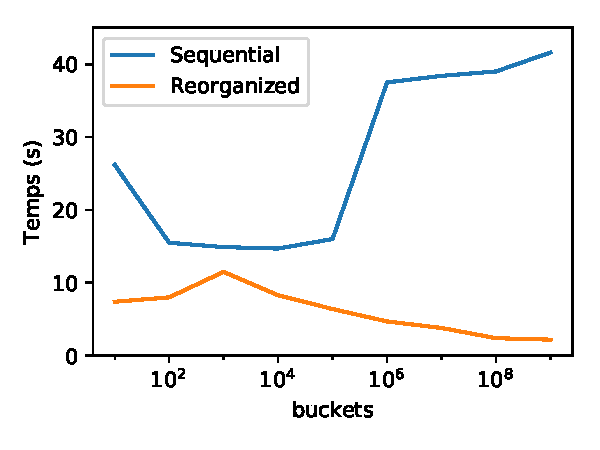
\includegraphics[width=\textwidth]{bucket.pdf}};
    \node at (0, 4) {$N = 10^{10}$};

    \draw[ultra thick,red,->] (-3, -3.75) node[red,left]{$\times 19$}  -| (4.45, -2.1);
  \end{tikzpicture}
\end{frame}

%%%%%%%%%%%%

\begin{frame}[label=radix_code]
  \frametitle{Un tableau d'entiers à trier ?}
  
    \begin{center}
      \Huge \bf \alert{Pro Tip}
  \end{center}

  \begin{exampleblock}{Algorithme de tri parallèle efficace}
    \begin{itemize}
  \item \emph{Parallel Bucket Sort} sur les 8 bits de poids forts
  \item Pour $0 \leq i < 2^8$, faire (en parallèle) :
    \begin{itemize}
    \item Trier le $i$-ème Bucket (avec un tri séquentiel normal)
    \end{itemize}
  \end{itemize}
\end{exampleblock}
  
\end{frame}


%%%%%%%%%%%%%%%%%%%%%%%%%%%%%%%%%%%%%%%%%%%%%%%%%%%%%%%%%%%%%%%%%%%%%%%%%%%%%%%%%%%%%

\subsection{Sparse LU}

%%%%%%%%%%%%%%%%%%%%%%%%%%%%%

\begin{frame}
  \frametitle{Idée générale n\textdegree 2 : procéder par \og phases\fg{}}

  \begin{columns}[c]
    \begin{column}{.1\textwidth}
      \vspace{1mm}
      \includegraphics[width=\textwidth]{triste.png}
    \end{column}
    
    \begin{column}{.9\textwidth}
      \begin{itemize}
      \item Accepter une réduction du degré de parallélisme...
      \end{itemize}
    \end{column}
  \end{columns}

  \vspace{1cm}
  
  \begin{columns}[c]
    \begin{column}{.1\textwidth}
      \vspace{3mm}
      
\includegraphics[width=\textwidth]{Content.png}
    \end{column}
    
    \begin{column}{.9\textwidth}
      \begin{itemize}
      \item ... Pour éliminer complètement les conflits
      \end{itemize}
    \end{column}
  \end{columns}  
\end{frame}

%%%%%%%%%%%%%%%%%

\begin{frame}[label=sparse_lu_intro]
  \frametitle{Exemple : factorisation LU creuse}

  \begin{center}
    \begin{tikzpicture}
      \path[red, dashed, use as bounding box] (0.25, -0.2) rectangle +(11, 3.6);

    % L en haut
    \begin{scope}  
      \node[anchor=south west, inner sep=0] at (0, 0)
      {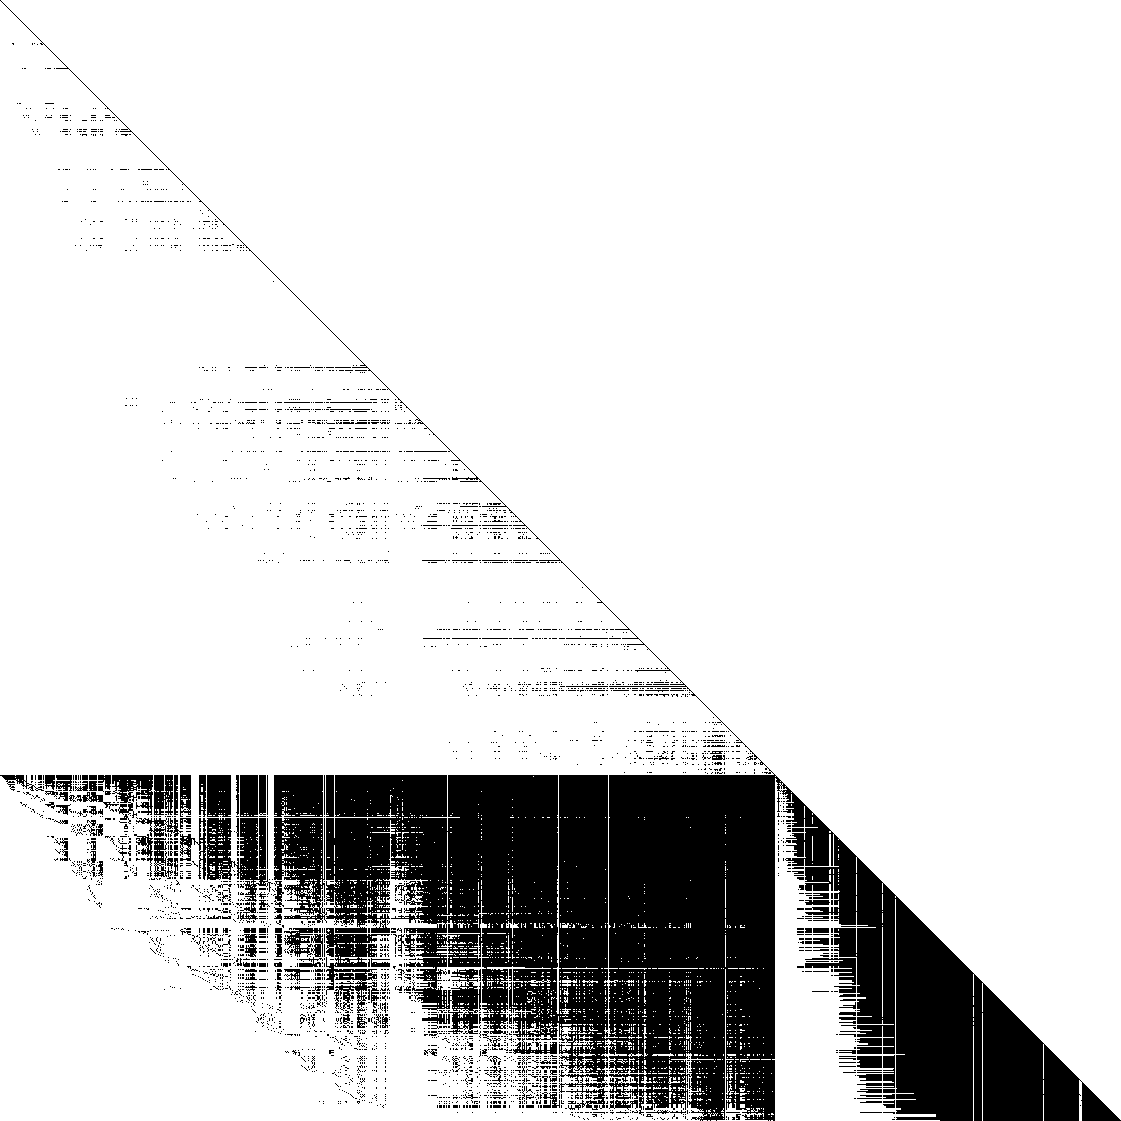
\includegraphics[width=2.8cm, height=3.25cm]{L}};
      \tikzmat{0,0}{2.8cm, 3.25cm}
    \end{scope}

    % U en haut
    \begin{scope}[xshift=3.1cm, yshift=0.45cm]
       \node[anchor=south west, inner sep=0] at (0, 0) {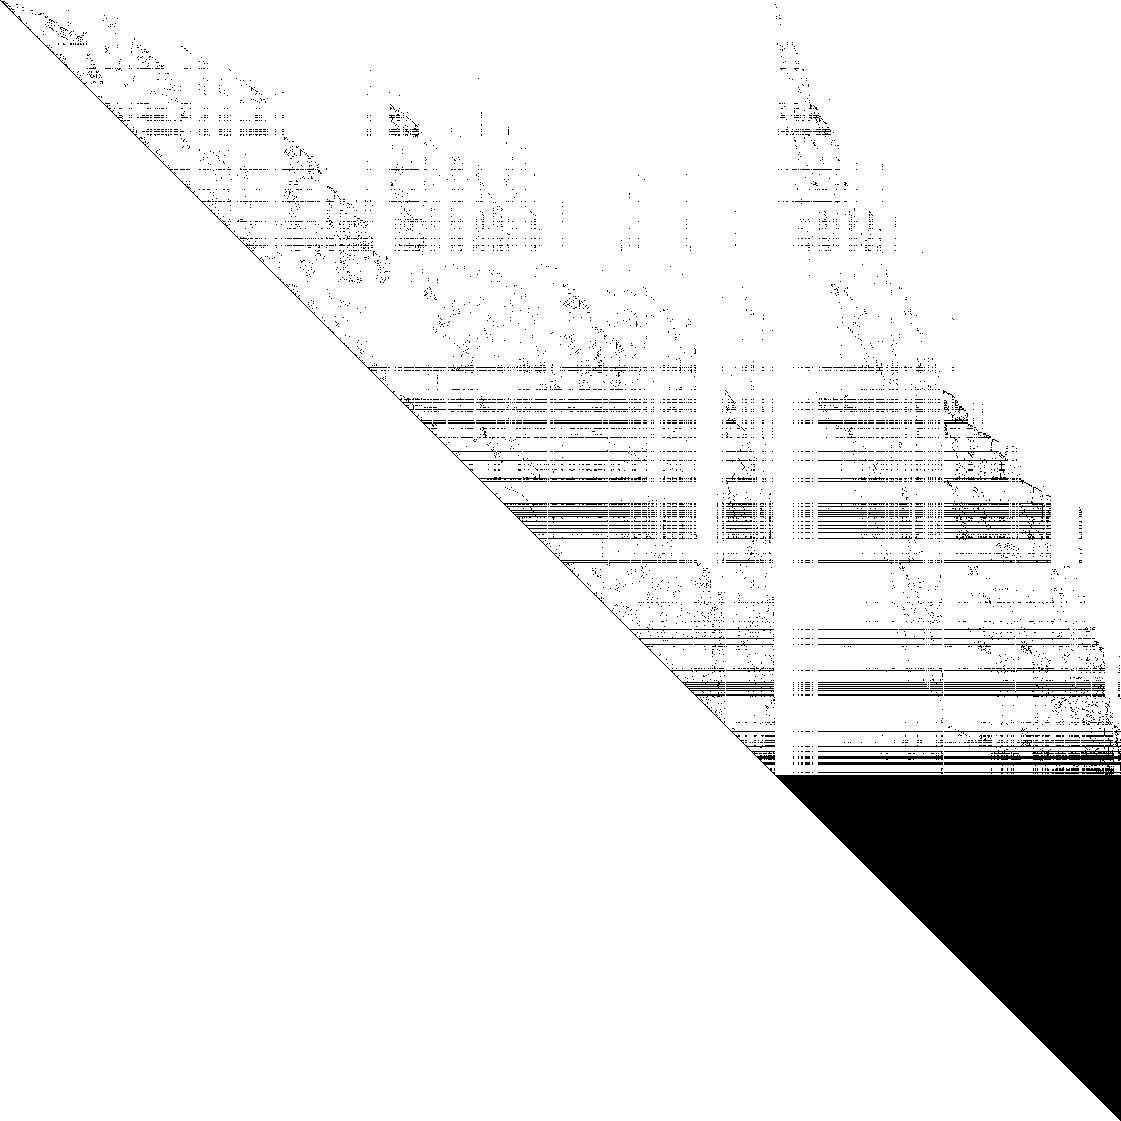
\includegraphics[width=2.8cm]{U}};
       \tikzmat{0,0}{2.8cm, 2.8cm}
     \end{scope}
    
    \node[anchor=west, font=\large] at (6, 1.6) {$= P \times$};

     \begin{scope}[xshift=7.4cm]
       \node[anchor=south west, inner sep=0] at (0, 0) {
\includegraphics[width=2.8cm, height=3.2cm]{tf13}};
       \tikzmat{0,0}{2.8, 3.2}
     \end{scope}

    \node[anchor=west, font=\large] at (10.25, 1.6) {$\times Q^{-1}$};
  \end{tikzpicture}
\end{center}
\end{frame}

%%%%%%%%%%%%%%%%%%%%%%%%%%%%%


\begin{frame}[label=sparse_lu_example]
  \frametitle{Exemple : factorisation LU creuse}

  \begin{columns}
    \begin{column}{3.4cm}
      \begin{tikzpicture}[every node/.style={font=\tiny},scale=0.4]
    % état initial aléatoire
    \pgfmathdeclarerandomlist{MyRandomColors}{{white}{white}{white}{white}{white}{white}{lightgray}}
    \foreach \i in {0, 1, ..., 49} {
      \pgfmathsetseed{55+\i}
      \foreach \j in {0, 1, ..., 49} {
          \pgfmathrandomitem{\RandomColor}{MyRandomColors} 
          \fill[fill=\RandomColor] (0.2*\j, 0.2*\i) rectangle +(0.2, 0.2);
        }
      }
      % cheat because I made a mistake
      \fill[fill=lightgray] (0, 0.2*48) rectangle +(0.2, 0.2);
      
      % pivot et ligne pivotale
      \foreach \j in {4, 5, 10, 26, 36, 39, 46} {
        \fill<2->[fill=blue] (0.2*\j, 0.2*48) rectangle +(0.2, 0.2);
      }
      \fill<2->[fill=red] (0, 0.2*48) rectangle +(0.2, 0.2);

      % colonne pivotale
      \foreach \i in {44, 37, 30, 23, 16, 9, 2} {
        \fill<2->[fill=blue] (0, 0.2*\i) rectangle +(0.2, 0.2);
      }

      \foreach \step / \i in {3/44, 4/37, 5/30, 6/23, 7/16, 8/9, 9/2} {
        %  étape d'élimination
        \fill<\step->[fill=white] (0, 0.2*\i) rectangle +(0.2, 0.2);
        \fill<\step->[fill=blue] foreach \j in {4, 5, 10, 26, 36, 39, 46} {(0.2*\j, 0.2*\i) rectangle +(0.2, 0.2)};
      }
      \path[use as bounding box] (5mm, 0) rectangle +(10, 10);
      \draw[use as bounding box] (0, 0) rectangle +(10, 10);
    \end{tikzpicture}
  \end{column}
  \begin{column}{6.5cm}
    \begin{alertblock}<10->{Plusieurs colonnes en parallèle ?}
      \begin{itemize}
      \item Conflit d'accès aux lignes !
      \end{itemize}
    \end{alertblock}

    \medskip
    
    \begin{exampleblock}<11->{Solution}
      Identifier DES colonnes \emph{indépendantes}.
    \end{exampleblock}
  \end{column}
\end{columns}

\begin{block}{Algorithme}
  \setlength{\leftmargini}{5mm}
  \begin{enumerate}
  \item~[Début.] $j \gets 1$
  \item~[Pivot.] Trouver $i$ avec $M_{ij} \neq 0$
  \item~[Élimination.] Pour $M_{i'j} \neq 0$ avec $i' \neq i$, faire $M_{i'} \gets (...) \times M_i$.
  \item~[Boucle.] Incrémenter $j$. Si $j=n$, STOP. Sinon retourner en 2.
  \end{enumerate}
\end{block}
\end{frame}

%%%%%%%%%%%%%%%%%%%%%%%%%%%%%%%%%%

\begin{frame}[label=sparse_lu_MIS]
  \frametitle{Exemple : factorisation LU creuse}

  \begin{columns}
    \begin{column}{0.4\textwidth}
  \begin{tikzpicture}[scale=0.8]
    \draw[red,thick,dashed] (0.5, -1) -- (0.5, 6) node[above] {$j$};
    \draw[red,thick,dashed] (2.5, -1) -- (2.5, 6) node[above] {$j'$};

    \draw[red,thick,dashed] (-1, 0.5) -- (4, 0.5) node[right] {$i$};
    
    \draw[fill=lightgray] (0, 0) rectangle +(1, 1);
    \draw[fill=lightgray] (2, 0) rectangle +(1, 1);
    \draw[fill=lightgray] (0, 2) rectangle +(1, 1);
    \draw[fill=lightgray] (2, 4) rectangle +(1, 1);
  \end{tikzpicture}
  
\end{column}
\begin{column}{0.6\textwidth}
  \begin{alertblock}{Dépendences}
    \begin{itemize}
    \item Colonnes $j$ et $j'$ liées par ligne $i$.
    \end{itemize}
  \end{alertblock}

  \medskip

  \begin{block}{Graphe de dépendence $G_{dep}$}
    \begin{itemize}
    \item Sommets $V = $ ens. des colonnes.
    \item Arêtes :
      \[
        E = \{ j \leftrightarrow j'~:~ \exists i. M_{ij} \neq 0 \wedge M_{ij'} \neq 0 \}.
      \]
    \end{itemize}
  \end{block}

  \begin{exampleblock}{Colonnes indépendantes}
    $\rightarrow$ Ensemble indépendant dans $G_{dep}$.
  \end{exampleblock}
\end{column}
\end{columns}
\end{frame}

%%%%%%%%%%%%%%%%%%%%%%%%%%%%%%%%%%%%%%%%%

\begin{frame}[label=sparse_lu_MIS]
  \frametitle{Exemple : factorisation LU creuse}

  \begin{block}{Nouvel algorithme :}
  \begin{itemize}
  \item Tant que ce n'est pas fini :
    \begin{itemize}
    \item Trouver un ensemble indépendant $\mathcal{I}$ dans $G_{dep}$.
      \begin{itemize}
      \item (optimal = NP-dur. Ici : algorithme glouton séquentiel)
      \end{itemize}
    \item Éliminer toutes les colonnes de $\mathcal{I}$ \alert{en parallèle}.
    \item \og Oublier\fg{} les colonnes éliminées
    \end{itemize}
  \end{itemize}
\end{block}

\bigskip

    \begin{columns}[c]
    \begin{column}{.1\textwidth}
      
\includegraphics[width=\textwidth]{Content.png}
    \end{column}
    \begin{column}[c]{.9\textwidth}

      Pas de conflit !
      
    \end{column}
  \end{columns}

  \bigskip
  
  \begin{columns}[c]
    \begin{column}{.1\textwidth}
      \includegraphics[width=\textwidth]{triste.png}
    \end{column}
    \begin{column}[c]{.9\textwidth}

      Portion séquentielle...
      
    \end{column}
  \end{columns}
\end{frame}


%%%%%%%%%%%%%%


\begin{frame}[label=sparse_lu_MIS_3]
  \frametitle{Exemple : factorisation LU creuse}
  \framesubtitle{Sous-exemple : algorithme glouton pour trouver un ensemble indépendant maxim\alert{al}}
  
  \begin{block}{Algorithme (implantable en temps linéaire)}
    \begin{itemize}
    \item $\mathcal{I} \gets \emptyset$
    \item Tant que $G$ n'est pas vide :
      \begin{itemize}
      \item Choisir un sommet $x$ quelconque.
      \item Ajouter $x$ à $\mathcal{I}$.
      \item Retirer $x$ et tous ses voisins de $G$.
      \end{itemize}
    \item Renvoyer $\mathcal{I}$.
    \end{itemize}
\end{block}

\bigskip

\begin{tikzpicture}[every node/.style={draw,shape=circle}]
  \node[] (a) at (0,0)  {A};
  \node[thick,text=red,right=of a] (b) {B};
  \node[thick,text=red,right=of b] (c) {C};

  \node[thick,text=green] at (5,0) (e) {A};
  \node[right=of e] (f) {B};
  \node[right=of f] (g) {C};
  \node[thick,text=green,right=of g] (h) {D};

  \draw (a) edge (b);
  \draw (b) edge[ultra thick] (c);

  \draw (e) edge (f);
  \draw (f) edge (g);
  \draw (g) edge (h);
\end{tikzpicture}

  \bigskip
  
  \begin{columns}[c]
    \begin{column}{.1\textwidth}
      \includegraphics[width=\textwidth]{triste.png}
    \end{column}
    \begin{column}[c]{.9\textwidth}

      En parallèle : conflit avec ses voisins...
      
    \end{column}
  \end{columns}
\end{frame}

%%%%%%%%%


\begin{frame}[label=parallel_MIS]
  \frametitle{Exemple : factorisation LU creuse}
  \framesubtitle{Sous-exemple : algorithme glouton pour trouver un ensemble indépendant maxim\alert{al}}

  \begin{exampleblock}{Algorithme modifié}
    \begin{itemize}
    \item $\mathcal{I} \gets \emptyset$
    \item Choisir une permutation aléatoire $\pi$ (\og \emph{score}\fg{}) de $\{1, \dots, n\}$.
    \item Tant que $G$ n'est pas vide : \uncover<2>{\hfill(\alert{\emph{$\approx \log^2 n$ iterations}})}
      \begin{itemize}
      \item $X = \{ u \in V~|~\text{$\pi[u] > \pi[v]$ pour tout $u \leftrightarrow v$} \}$ %$
      \item Ajouter $X$ à $\mathcal{I}$.
      \item Retirer $X$ et tous les voisins des sommets de $X$ de $G$.
      \end{itemize}
    \item Renvoyer $\mathcal{I}$.
    \end{itemize}
  \end{exampleblock}
  
\bigskip

\begin{tikzpicture}[every node/.style={draw,circle solidus,font=\scriptsize,inner sep=0pt}]
  \node[thick,text=red] (a) at (0,0)  {A \nodepart{lower} 50};
  \node[right=of a] (b) {B \nodepart{lower} 30};
  \node[thick,text=red,right=of b] (c) {C \nodepart{lower} \alert{64}};

  \node[] at (5,0) (e) {A \nodepart{lower} 10};
  \node[right=of e] (f) {B \nodepart{lower} 20};
  \node[right=of f] (g) {C \nodepart{lower} 30};
  \node[thick,text=red,right=of g] (h) {D \nodepart{lower} 40};

  \draw (a) edge[] (b);
  \draw (b) edge[very thick] (c);

  \draw (e) edge[very thick] (f);
  \draw (f) edge (g);
  \draw (g) edge[very thick] (h);
\end{tikzpicture}

\end{frame}

%%%%%%%%%%%%%%%%%

\section{Tricks transactionnels}

\begin{frame}[label=transactions]
  \frametitle{Transactions parallèles}

  \textbf{lecture} $A[i_1], A[i_2], \dots$ $\rightarrow$ \textbf{calcul} $\rightarrow$ \textbf{écriture} $A[k_1], A[k_2], \dots$.

  \medskip

  \begin{block}{Obstacle à l'exécution \og atomique\fg{} :}
    \begin{itemize}
    \item Les données lues ont été modifiées avant l'écriture.
    \item Résultat du calcul \og périmé\fg{}.
    \end{itemize}
  \end{block}
  
  \begin{overlayarea}{\textwidth}{4cm}
  \begin{alertblock}<only@1>{\textbf{Approche pessimiste} (\og \textit{Ask for Permission}\fg{})}
    \begin{itemize}
    \item \og Verrouiller\fg{} les données lues.
    \item Lecture/Verrouillage $\rightarrow$ Calcul $\rightarrow$ écriture $\rightarrow$ déverrouillage
      \begin{itemize}
      \item Bloque modification \textbf{potentielle} par un autre thread.
      \end{itemize}
    \item Faire comme si le conflit \textbf{ALLAIT} avoir lieu.
    \item Surcoût inutile en l'absence de conflit.
    \end{itemize}
  \end{alertblock}

  \begin{exampleblock}<only@2>{\textbf{Approche optimiste} (\og \textit{Shoot First, Ask Questions Later}\fg{})}
    \begin{itemize}
    \item Lire (\alert{sans précaution !!!}) $\rightarrow$ Calcul $\rightarrow$ \textbf{Commit} (atomique) :
      \begin{itemize}
      \item Vérifier la fraîcheur des données lues,
      \item Si OK, effectuer l'écriture ; sinon, tout recommencer.
      \end{itemize}
    \item Faire comme si le conflit \textbf{N'ALLAIT PAS} avoir lieu.
    \item Travail perdu en cas de conflit.
    \end{itemize}
  \end{exampleblock}    
\end{overlayarea}
\end{frame}

% technique de versioning : couplages sans cycles alternants
%%%%%%%%%%%%%%%%%%%%%%%%%%%%%%%%%%%%%%%%%%%%%%

\begin{frame}[label=idea1]
  \frametitle{Idée générale : \textbf{analyser la fréquence des conflits}}

  \begin{columns}[c]
    \begin{column}{.1\textwidth}
      \vspace{1mm}
      \includegraphics[width=\textwidth]{triste.png}
    \end{column}
    
    \begin{column}{.9\textwidth}
      \begin{itemize}
      \item Prendre le risque de gâcher un peu de calcul...
      \end{itemize}
    \end{column}
  \end{columns}

  \vspace{1cm}
  
  \begin{columns}[c]
    \begin{column}{.1\textwidth}
      \vspace{3mm}
      
\includegraphics[width=\textwidth]{Content.png}
    \end{column}
    
    \begin{column}{.9\textwidth}
      \begin{itemize}
      \item ... Pour réduire le coût de la gestion des conflits
      \end{itemize}
    \end{column}
  \end{columns}  
\end{frame}

%%%%%%%%%%%%%%%%%%%%%%%%%%%%%%%%%%%%%%%%%%%%%%

\begin{frame}[label=versioning]
  \frametitle{Technique générale : le \emph{versioning}}

  \begin{itemize}
  \item Structure de donnée partagée, avec un \alert{numéro de version}
  \item $v = 0$ au début (\alert{impair} pendant les écritures).
  \end{itemize}

  \begin{alertblock}{Écrivain}
    \begin{enumerate}
    \item Entrer section critique ; incrémenter $v$
    \item Effectuer les écritures
    \item incrémenter $v$ ; sortir section critique.
    \end{enumerate}
  \end{alertblock}

  \begin{exampleblock}{Lecteur}
    \begin{enumerate}
    \item $v_{before} \gets v$
    \item Effectuer lectures
    \item $v_{after} \gets v$
    \item Si $v_{before}$ impair ou $v_{before} \neq v_{after}$, recommencer.
    \end{enumerate}
  \end{exampleblock}  
\end{frame}

%%%%%%%%%%%%%%%%%% 

\begin{frame}
    \frametitle{Technique générale : le \emph{versioning}}

    \begin{center}
      \begin{tikzpicture}[scale=0.9, every node/.style={font=\small}]
        \foreach \i in {0, 1, 2, 3} {
          \node at (-0.5, 0.5 + \i)  {$T_\i$};
        }
        \node at (-0.5, -0.5)  {$T_w$};
        \draw[dashed] (3, -1.5) -- +(0, 5.75);
        \draw[dashed] (8, -1.5) -- +(0, 5.75);
        
  % lectures avant
  \draw[fill=white] (0.5, 1) rectangle node {reads} +(1, 0.75);
  \draw[fill=white] (0.75, 3) rectangle node {reads} +(1, 0.75);  
  
  % lecture échouent 
  \draw[fill=gray] (2, 0) rectangle node {reads} +(4, 0.75);
  \draw[fill=gray] (2.5, 1) rectangle node {reads} +(5, 0.75);
  \draw[fill=gray] (1, 2) rectangle node {reads} +(3, 0.75);
  \draw[fill=gray] (2.5, 3) rectangle node {reads} +(2, 0.75);
  \draw[fill=gray] (7, 0) rectangle node {reads} +(2, 0.75);
  \draw[fill=gray] (5, 2) rectangle node {reads} +(1, 0.75);
  \draw[fill=gray] (7, 2) rectangle node {reads} +(3, 0.75);
  \draw[fill=gray] (5, 3) rectangle node {reads} +(4, 0.75);

  % lectures après
  \draw[fill=white] (9.5, 0) rectangle node {reads} +(1, 0.75);  
  \draw[fill=white] (8.5, 1) rectangle node {reads} +(1, 0.75);
  \draw[fill=white] (10.5, 2) rectangle node {reads} +(1, 0.75);  
  \draw[fill=white] (10, 3) rectangle node {reads} +(1, 0.75);

  % thread écrivain
  \draw[fill=yellow] (3.25, -1) rectangle node[] {write} +(4.5, 0.75);
\end{tikzpicture}
\end{center}

\begin{itemize}
\item Écrivains prioritaires sur les lecteurs
\end{itemize}


\end{frame}

%%%%%%%%%%%%%%%%%%%%%%%%%%%%%%%%%%%%%%%%%%%%%%%

\begin{frame}[label=urmatching]
  \frametitle{Exemple : plus grand couplage sans cycle alternant}

  \begin{center}
  \begin{tikzpicture}[xscale=1.41,>=stealth,yscale=1.2]

\node at (0, 2) (R1) {A};
\node at (0, 1) (R2) {B};
\node at (0, 0) (R3) {C};
\node at (1,2) (C1) {1};
\node at (1,1) (C2) {2};
\node at (1,0) (C3) {3};
\draw[blue] (C1) edge (R2);
\draw[blue] (C2) edge (R1);
\draw(R2)--(C3);
\draw[red,very thick] (R1) edge (C1);
\draw[red,very thick] (R2) edge (C2);
\draw[very thick](R3)--(C3);
\draw (C3) +(-0.5, -0.2) node[align=center,below,font=\footnotesize]{Couplage avec \red{\textbf{c}}\blue{y}\red{\textbf{c}}\blue{l}\red{\textbf{e}} \blue{a}\red{\textbf{l}}\blue{t}\red{\textbf{e}}\blue{r}\red{\textbf{n}}\blue{a}\red{\textbf{n}}\blue{t} \\ (polynomial)};


\begin{scope}[xshift=4cm]
  \node at (0, 2) (RR1) {A};
\node at (0, 1) (RR2) {B};
\node at (0, 0) (RR3) {C};
\node at (1,2) (CC1) {1};
\node at (1,1) (CC2) {2};
\node at (1,0) (CC3) {3};
\draw (CC1) edge (RR2);
\draw (RR1) edge (CC2);
\draw[very thick] (CC1) edge (RR1);
\draw[very thick] (RR2) edge (CC3);
\draw (RR1) edge (CC1);
\draw (RR2) edge (CC2);
\draw (RR3) edge (CC3);
\draw (CC3) +(-0.5, -0.2) node[below,font=\footnotesize,align=center]{Couplage sans cycle alternant \\ (NP-dur)};
\end{scope}
\end{tikzpicture}
\end{center}

\begin{block}{Algorithme glouton \uncover<2>{parallèle avec \textbf{\bfseries Versioning}}}
  Pour tout sommet $u$ (en parallèle) et toute arête $(u \leftrightarrow v)$  :
  \begin{itemize}
  \item<2-> $t \gets |\mathcal{C}|$ 
  \item Parcours en largeur \blue{a}\red{\textbf{l}}\blue{t}\red{\textbf{e}}\blue{r}\red{\textbf{n}}\blue{a}\red{\textbf{n}}\blue{t} depuis $u$ ; atteint $v$ ? $\Rightarrow$ \texttt{abort}.
  \item<only@1> Ajoute $(u \leftrightarrow v)$ à $\mathcal{C}$. \hfill \textit{[OK, pas de cycle]} 
  \item<only@2> \textbf{section critique} : si $t = |\mathcal{C}|$, ajoute $(u \leftrightarrow v)$ à $\mathcal{C}$ ; ok $\gets 1$.
  \item<2> Si $ok = 0$, recommencer.\hfill\textit{[KO, couplage modifié]} 
  \end{itemize}
\end{block}
\end{frame}

%%%%%%%%%%%%%%%%%%%%%%%%%%%%%%

\section{Support Hardware pour la concurrence}

\begin{frame}[fragile, label=rtm]
  \frametitle{Concept de \og transaction \fg{}}

  \begin{itemize}
  \item Problèmes similaires dans les serveurs de bases de données
  \item Nombreuses techniques de gestion des transactions
  \end{itemize}

  \begin{columns}
    \begin{column}{0.47\textwidth}
  \begin{alertblock}{CPU (très) modernes :\\ \textbf{transactional memory}}
\begin{minted}{C}
#include <immintrin.h>
unsigned int status = _xbegin();
if (status == _XBEGIN_STARTED) {
    // Access shared data ...
    if (problem)    // give up ?
        _xabort(0); 
    // Access more shared data ...
    _xend();
    /* <-------- Success !!! */
} else { /* <--- Failure */
    if (status & _XABORT_EXPLICIT)
        ...
    if (status & _XABORT_CONFLICT)
        ...    
    if (status & _XABORT_CAPACITY)
        ...
}
\end{minted}
  \end{alertblock}
\end{column}
\begin{column}{0.63\textwidth}
  \begin{itemize}
  \item \verb|_xbegin()| démarre une transaction
    \begin{itemize}
    \item Renvoie \verb|_XBEGIN_STARTED|
    \item Purge le cache...
    \end{itemize}
  \item \verb|_xend()| tente le \og commit\fg{}.
    \begin{itemize}
    \item OK $\rightarrow$ l'exécution continue.
    \end{itemize}
  \item \verb|_xabort(cst)| force l'échec

    \medskip

  \item \alert{En cas d'échec} :
    \begin{itemize}
    \item Retourne après \verb|_xbegin()|
    \item Code erreur (conflit, resources, ...)
    \end{itemize}

    \medskip

  \item Toujours pas la panacée
    \begin{itemize}
    \item Coût non-négligeable
    \item Faux-positifs, ...
    \end{itemize}

    \medskip

  \item Cf. aussi bibliothèque \texttt{TinySTM}
  \end{itemize}
\end{column}
\end{columns}
\end{frame}

%%%%%%%%%%%%%%%%%%%%%%%%%%%%%%%%%%%%%%%%

\begin{frame}[fragile, label=CAS]
  \frametitle{L'opération \emph{Compare-And-Swap}}

  \small
  \begin{itemize}
  \item OpenMP spécifie un \emph{modèle mémoire} et des \emph{opérations
      atomiques} séquentiellement consistantes.
  \item \textbf{C11} (ISO/IEC 9899:2011) donne des équivalents.
  \item Avec un (gros) bonus : \textbf{\emph{compare-and-swap} \alert{atomique}}.
  \end{itemize}

\medskip
  
\begin{minted}{C}
#include <stdatomic.h>
bool atomic_compare_exchange_strong(volatile A* obj, C* expected, C desired);
bool atomic_compare_exchange_weak(volatile A *obj, C* expected, C desired);
\end{minted}

\medskip

\begin{block}{Spécification --- version \emph{strong}}
  \mintinline{C}{ok = (obj == expected); if (ok) obj = desired; return ok}% \hfill\alert{(atomique !)}
\end{block}

\medskip

\begin{enumerate}
\item Instruction du CPU (ou versions équivalents LL/SC)
\item La version \emph{weak} peut avoir des faux négatifs
\end{enumerate}

\end{frame}

%%%%%%%%%%%%%%%%%%%%%%%%%%

\begin{frame}[fragile]
  \frametitle{Et dans OpenMP ?}

  \begin{columns}[b]
    \begin{column}{.1\textwidth}
      
\includegraphics[width=\textwidth]{Content.png}
    \end{column}
    \begin{column}{.9\textwidth}
      \begin{itemize}
      \item Compare-and-swap est dans OpenMP 5.1
      \item Paru en novembre 2020
      \end{itemize}
    \end{column}
  \end{columns}

\bigskip
  
\begin{minted}[fontsize=\normalsize]{C}
#pragma omp atomic compare
if (obj == expected)
        obj = desired;

#pragma omp atomic compare capture
if (obj == expected)
        obj = desired;
else
        v = obj;
\end{minted} 

\bigskip

\begin{columns}[b]
    \begin{column}{.1\textwidth}
      
\includegraphics[width=\textwidth]{Triste.png}
    \end{column}
    \begin{column}{.9\textwidth}
      \begin{itemize}
      \item \texttt{gcc} 10.2 ne l'implante pas encore...
      \end{itemize}
    \end{column}
  \end{columns}

\end{frame}

%%%%%%%%%%%%%%%%%%%%%%%%%%

\begin{frame}[fragile, label=CAS]
  \frametitle{Transactions avec \emph{Compare-And-Swap}}

  On peut faire (presque) n'importe quoi avec \emph{Compare-And-Swap} !

  \bigskip
  
  \begin{block}{Idée générale : \emph{Compare-And-Swap Loop}}
    \begin{enumerate}
    \item~[Begin.] $x_{old} \gets x$ 
    \item~[Work.] Calculer une mise à jour $x_{new}$
    \item~[Commit.] \mintinline{C}{ok = atomic_compare_exchange_strong(x, x_old, x_new)}
    \item~[Repeat.] Si pas \texttt{ok}, retourner en 1.
      \end{enumerate}
    \end{block}
  \end{frame}
  
\begin{frame}[fragile, label=CAS_list]
  \frametitle{Exemples avec \emph{Compare-And-Swap}}

  \begin{exampleblock}{Exemple : liste chainée}
\begin{minted}{C}
struct item_t {
    ...
    struct item_t *next;
}

void atomic_append(struct item_t *list, ...)
{
    struct item_t *new =  malloc(sizeof(*new));
    ...
    bool ok = false;
    while (!ok) {
        new->next = list;
        ok =  atomic_compare_exchange_strong(list, new->next, new);
    }
}
\end{minted}
    \end{exampleblock}
\end{frame}

%%%%%%%%%%%%%%%%%%%%%%%%

\begin{frame}[fragile, label=CAS_hash]
  \frametitle{Exemples avec \emph{Compare-And-Swap}}

  \begin{exampleblock}{Exemple : table de hachage avec sondage linéaire}
\begin{minted}{C}
void insert(void *H, void *item)
{
    int i = hash_function(item);        // hash
    while (H[i] != EMPTY)               // trouve une case vide
        i = (i + 1) % HASHTABLE_SIZE;        
    H[i] = item;                        // insert
}
\end{minted}
  \end{exampleblock}

\medskip
  
  \begin{alertblock}{Version thread-safe}
\begin{minted}{C}
void ATOMIC_insert(void *H, void *item)
{
    int i = hash_function(item);
    book ok = false
    while (!ok) {
        ok = atomic_compare_exchange_strong(H[i], EMPTY, item);
        i = (i + 1) % HASHTABLE_SIZE;        
    }
}
\end{minted}
  \end{alertblock}
\end{frame}

%%%%%%%%%%%%%%%%%%%%%%%%%%%%%%%%%%%%%%%%%%%%%%%%%%%%%%%%%%

\begin{frame}[label=lock-free-defs]
  \frametitle{Idée générale : algorithmes \emph{lock-free}}

  \begin{block}{Définition}
    Une fonction est \textbf{lock-free} si, lorsqu'elle est appelée par plusieurs
    threads à la fois, au moins l'une des invocations termine en un nombre fini
    d'étapes de calcul (quoi que fassent les autres, même s'ils bloquent).
  \end{block}

  \bigskip
  
  Remarque : si une fonction acquiert un verrou / section critique, elle ne peut
  pas être \emph{lock-free}.

  \pause\bigskip
  
  \begin{tikzpicture}
    \node (switch) {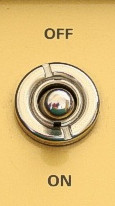
\includegraphics[width=2cm]{switch.jpg}};
    \node[above right=-10mm and 0mm of switch, font={\Large\bfseries}] {Safety};
    \node[below right=-10mm and 0mm of switch, text=red, font={\Large\bfseries}] {World of PAIN};
    \node[left=of switch, font={\large}] (label) {Guru switch};
    \draw (label) edge[->] (switch);
  \end{tikzpicture}

\end{frame}

%%%%%%%%%%%%%%%%%%%%%%%%%%%%%%%%%%%%%%%%%%%%%%%%%%%%%%%%%

\begin{frame}[fragile,label=seq_intset]
  \frametitle{Exemple : ensemble d'entiers}

  \begin{tabular}{c|c}
\begin{minipage}[t]{0.55\textwidth}
\begin{minted}[fontsize=\scriptsize]{C}
bool * A;   
int N, min;  

// A[i] indique si i est dans l'ensemble
// min pointe sur le plus petit élément

void setup()
{
   A = malloc((N + 1) * sizeof(*A));
   // astuce : sentinelle en position N
   for (int i = 0; i < N + 1; i++)
      A[i] = true;
   min = 0;
}
\end{minted}
\end{minipage}
  &
\begin{minipage}[t]{0.45\textwidth}
\begin{minted}[fontsize=\scriptsize]{C}
bool remove(int i)
{
    bool x = A[i];
    A[i] = false;
    return x;
}

int extract_min()
{
   while(A[min] == false)
      min++;
   if (min < N)
      remove(min);
   return min;
}
\end{minted}
\end{minipage}
  \end{tabular}

\begin{alertblock}{Invariants}
  \texttt{A[N] == true} et \texttt{A[0:min] == false}.
\end{alertblock}
\end{frame}

%%%%%%%%%%%%%%%%%%%%%%%%%%%

\begin{frame}[fragile,label=lf_intset]
  \frametitle{Exemple : ensemble d'entiers \alert{lock-free}}
  
\begin{minted}[fontsize=\scriptsize]{C}
#include <stdbool.h>
#include <stdatomic.h>
#define CAS atomic_compare_exchange_weak

_Atomic bool * A;         
_Atomic int min;          
int N;
bool yes = true;

void setup()
{
    A = malloc((N + 1) * sizeof(*A));
    for (int i = 0; i < N + 1; i++)
        atomic_store(&A[i], true);
    atomic_store(&min, 0);
}

bool remove(int i)
{
    return atomic_exchange(&A[i], false);    // comme précédemment
}
\end{minted}
\end{frame}

%%%%%%%%%%%%%%%%%%%%%%%%%%%


\begin{frame}[fragile,label=lf_intset]

  \smallskip
  
\begin{alertblock}{Invariants}
  \texttt{A[N] == true} et \texttt{A[0:min] == false}.
\end{alertblock}

\begin{overlayarea}{\textwidth}{8cm}
\begin{minted}[fontsize=\scriptsize]{C}
int extract_min()
{
    int old_min = atomic_load(&min);
    int i = old_min;               // cherche A[i] == true
    while(atomic_load(&A[i]) == false)
        i++;
\end{minted}
\begin{onlyenv}<2->%
\begin{minted}[fontsize=\scriptsize]{C}
    if (i == N) {                  // ensemble vide ?
        atomic_store(&min, N);     
        return N;
     }
\end{minted}
\end{onlyenv}%
\begin{onlyenv}<3>
\begin{minted}[fontsize=\scriptsize]{C}
    atomic_store(&A[i], false);
  \end{minted}
  \begin{block}{Raté}
    \begin{itemize}
    \item On a bien vu \texttt{A[i] == true} ...
    \item ... mais ça a pu changer entre-temps ...
    \item Si un autre \texttt{extract\_min()} a eu lieu en même temps
    \end{itemize}
  \end{block}
\end{onlyenv}
\begin{onlyenv}<4->
\begin{minted}[fontsize=\scriptsize]{C}
    bool ok = CAS(&A[i], &yes, false);
    if (!ok)         
        return extract_min();      // A[i] == false ? On recommence   
\end{minted}
\end{onlyenv}
\begin{onlyenv}<5>
\begin{minted}[fontsize=\scriptsize]{C}
    CAS(&min, &old_min, i);        // avance min (paresseusement)
    return i;
}
\end{minted}
\end{onlyenv}
\begin{onlyenv}<6->
\begin{minted}[fontsize=\scriptsize]{C}
    while(old_min < i) {           // avance min (consciencieusement)
        bool ok = CAS(&min, &old_min, i);
        if (ok)
            break;
        old_min = atomic_load(&min);
    }
    return i;
}
\end{minted}
\end{onlyenv}
\end{overlayarea}

\end{frame}

%%%%%%%%%%%%%%%%%%%%%%%%%%%%%%%%

\begin{frame}[label=lf_intset]
  \frametitle{La question à 20\ 000 points}

  {\Huge Est-ce correct ?}

  \bigskip\pause

  \begin{alertblock}{Question subsidiaire}
    Que signifie \og être correct\fg{} ?
  \end{alertblock}

  \bigskip\pause
  
  \begin{exampleblock}{Définition}
    Une structure de donnée est \textbf{linéarisable} si tout se passe comme si les
    fonctions qui y accèdent prenaient effet \emph{instantanément}, à un point
    quelconque entre leur invocation et leur terminaison.
  \end{exampleblock}

  \bigskip\pause

  Correct $\approx$ linéarisable

  \bigskip\pause

  Exercice : faites la preuve.
\end{frame}


%%%%%%%%%%%%%%%%%%%%%%%%



\end{document}

%%% Local Variables:
%%% TeX-command-extra-options: "-shell-escape"
%%% TeX-engine: xetex
%%% End: